\documentclass[12pt]{report}   % SUBMISSION TO GRAD SCHOOL
%\documentclass[12pt,twoside]{report}  % TWOSIDE DUPLEX OUTPUT
\usepackage{setspace}
\usepackage{buthesis}
\usepackage{amsmath,amssymb,graphicx,amsfonts,amsthm}
\usepackage{verbatim}
\usepackage{epsfig}
\usepackage{wrapfig}
\usepackage{latexsym,amsfonts,amscd}
\usepackage{changebar}
\usepackage{enumerate}
\usepackage[table]{xcolor}
% Do you use TikZ?
\usepackage{tikz}
%\usepackage{pgfmath}
\usetikzlibrary{decorations}
\usetikzlibrary{shadows}

% Used only for example text
\usepackage{lipsum}

\usepackage[footnotesize,bf]{caption}  % Reduces caption font sizes
\usepackage{natbib}


\usepackage{amsmath}
\usepackage{amsfonts}
\usepackage{amssymb}
\usepackage{graphicx}
\usepackage{booktabs}
\usepackage{color}
\usepackage{longtable}
\usepackage{array}
\usepackage{amssymb}
%\usepackage[usenames,dvipsnames,svgnames,table]{xcolor}




%%%%%%%%%%%%%%%%% Fancy chapter headings %%%%%%%%%%%%%%%%%%%
\usepackage[Bjarne]{ThesisFncychap}
% Redefine alphano commands

%%%%%%%%%%%%%%%%%%%%%%%%%%%%%%%%%%%%%%%%%%%%%%%%%%%
\makeatletter
  
  \ChNameVar{\Huge\sc}    % sets the style for name
  \ChNumVar{\Huge\sc}         % sets the style for digit
  \ChTitleVar{\Huge\bf\centering} % sets the style for title
  \ChRuleWidth{4pt}        % Set RW=4pt
  %\ChNameUpperCase         % Make name uppercase
  \ChNameAsIs         % Make name uppercase
  \ChTitleAsIs

  \renewcommand{\DOCH}{%
    %\setlength{\fboxrule}{\RW} % Let fbox lines be controlled by
                               % \ChRuleWidth
    %\fbox{\CNV\FmN{\@chapapp}\space \CNoV\thechapter}\par\nobreak
    \thispagestyle{empty}
    \vskip 80\p@
    \begin{center}
    %\CNV\FmN{\@chapapp}\space \CNoV\thechapter\par\nobreak
    \CNV\FmN{\@chapapp} \TheAlphaChapter\par\nobreak
    \begin{tabular*}{\textwidth}{c}
      \hline
    \end{tabular*}
    %\line(1,0){5in}\\
    \end{center}
    %\vskip 20\p@
    }

  \renewcommand{\DOTI}[1]{%
    \CTV\FmTi{#1}\par\nobreak
    \vskip 40\p@
    {\newpage}
    }
  \renewcommand{\DOTIS}[1]{%
    \CTV\FmTi{#1}\par\nobreak
    \vskip 40\p@
    }
\makeatother


%%%%%%%%%%%%%%%%%%%%%%%%%%%%%%%%%%%%%%%%%%%%%%%%%%%%%%%%%%%%

%-----------------------------------------------------------------
%% Control the fonts and formatting used in the table of contents, list of
%% figures, and list of tables
\usepackage[titles]{tocloft}
%\newcommand{\del}{\partial}
\graphicspath{ {images/}{images/Growth_Rate_Cont_Plots/} }



\newcommand{\by}{\mathbf{y}}
\newcommand{\bx}{{\boldsymbol{\hat{x}}}}
\newcommand{\bn}{{\boldsymbol{\hat{n}}}}
\newcommand{\bt}{{\boldsymbol{\hat{t}}}}
\newcommand{\bu}{\mathbf{u}}
%\newcommand{\bn}{\mathbf{n}}
%\newcommand{\bt}{\mathbf{t}}
\newcommand{\grad}{\mathbf{\nabla}}
\newcommand{\del}{\partial}
\newcommand{\hg}{h_g}
\newcommand{\Rey}{{R}}
\newcommand{\Ndg}{\tilde{N}_g}
\newcommand{\monami}{\textit{monami}}
\newcommand{\ubl}{U_\text{bl}}
\newcommand{\words}[1]{\textbf{(#1)~}}
% \newcommand{\words}[1]{{}}
\newcommand{\ReyNdg}{{\Rey\Ndg}}


\renewcommand{\bar}{\overline}
\definecolor{tableShade}{gray}{0.8}
%% Aesthetic spacing redefines that look nicer to me than the defaults.
\setlength{\cftbeforechapskip}{-1ex}
\setlength{\cftbeforesecskip}{-3.5ex}
\setlength{\cftbeforesubsecskip}{-3.5ex}
\setlength{\cftbeforetabskip}{-3.5ex}
\setlength{\cftbeforefigskip}{-3.5ex}
%-----------------------------------------------------------------

\dissertation % This *is* what you're writing, right?

% Information about the document
%-----------------------------------------------------------------
\title{
Hydrodynamic instability leading to \textit{Monami}
}
\author{Ravi Shanker Singh}
\degree{Doctor of Philosophy}
\department{Department of Physics}
\previousdegrees{
		B.Sc., Banaras Hindu University; Varansi, India, 2006\\ 
		M.Sc.(Physics), Indian Institute of Technology-Bombay; Mumbai, India, 2008}	
\thesismonth{May} \thesisyear{2014}
%-----------------------------------------------------------------

\begin{document}

\doublespacing
\begin{preliminaries}
\maketitle

\copyrightpage

\begin{signature}
  \director{Shreyas Mandre, Ph.D., Advisor}
  \reader{J. Tang, Ph.D., Reader}
  \reader{Tom Powers, Ph.D., Reader}
\end{signature}

\begin{vita}
  %\lipsum[1-2]

  %xzczxl;csd ;vdfsvl;sd
\end{vita}

\begin{acknowledgments}
 % \lipsum[3-4]

\end{acknowledgments}

\begin{abstract}
 % \lipsum[6-8]

  \thispagestyle{empty}
  % Do you want this page to exist in the numbering?
%  \thispagestyle{empty}
%  \if@twoside
%    \addtocounter{page}{-2}  
%  \else
%    \addtocounter{page}{-1}
%  \fi
\end{abstract}

% Why double-space toc,lof, and lot?
\begin{spacing}{1}
  \tableofcontents
  \clearpage{\pagestyle{empty}\cleardoublepage}

  \footnotesize
  \fontsize{11.5pt}{12.5pt}\selectfont
  \listoftables
  \clearpage{\pagestyle{empty}\cleardoublepage}

  \listoffigures
  \clearpage{\pagestyle{empty}\cleardoublepage}
  \normalsize
\end{spacing}

\end{preliminaries}

\pagestyle{myheadings}

%------------------------ CONTENT ------------------------%

\chapter{Introduction}
\subsection{Motivation}
Seagrasses are submerged flowering plants found in shallow marine waters, mostly in the littoral zones of freshwater and in large expanses of low lying coastal shore, they occupy less than $0.05\%$ of the ocean area \cite{green2003world} but contribute directly to about $15\%$ of the total biomass production in the ocean \cite{duarte1999}. Seagrasses plays crucial role in protecting sea shores. The extensive root system in seagrasses, which extends both vertically and horizontally, helps stabilize the sea bottom in a manner similar to the way land grasses prevent soil erosion. With no seagrasses to diminish the force of the currents along the bottom, numerous beaches, businesses, and homes can be subject to greater damage from storms.
%ocean bottom areas which are mostly devoid of seagrass are vulnerable to intense wave action from currents and storms. 

Seagrasses provide food, shelter, and essential nursery areas to commercial and recreational fishery species and to countless invertebrates living in seagrass communities.
Some fish, such as seahorses and lizardfish, can be found in seagrasses throughout the year, while other fish spends their certain life stages in seagrass beds. While some organisms, including the endangered Florida manatee and green sea turtle, graze directly on seagrass leaves, others use seagrasses indirectly for nutrients. Bottlenose dolphins are often found feeding on organisms that live in seagrass areas. Detritus from bacterial decomposition of dead seagrass plants provides food for worms, sea cucumbers, crabs, and filter feeders such as anemones and ascidians. Further decomposition releases nutrients (such as nitrogen and phosphorus), which, when dissolved in water, are re-absorbed by seagrasses and phytoplankton.
\begin{figure}
\centerline{ 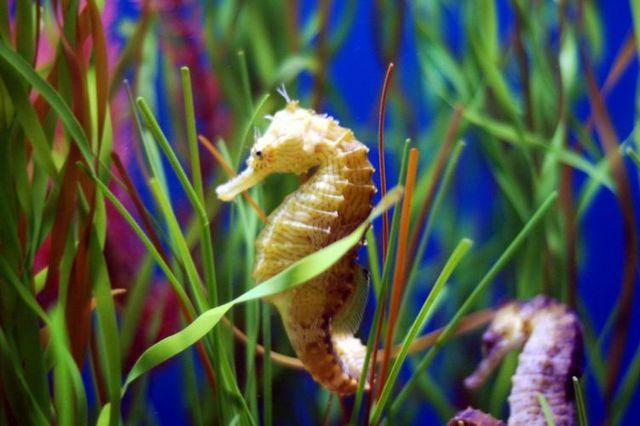
\includegraphics[scale=1.45]{SeaHorse} \includegraphics[scale=0.045]{GreenSeaTurtle} }
\caption{Seahorse (left) uses seagrass for their habitat and Green sea turtle (right) grazing on seagrass leaves, pictures taken from \textit{amagintheseaworldpress.com} and  \textit{mikegil.com} respectively  }
\end{figure}

The relative safety of seagrass meadows from strong water current provides an ideal environment for the female fishes to to lay and hatch their eggs \cite{rooker98}. The safety of seagrass meadows are also useful for the juvenile fish and invertebrates to hide themselves from predators. Seagrass leaves are also ideal for the attachment of larvae and eggs, including those of the sea squirt and mollusk. Much of Florida's recreationally and commercially important marine life can be found in seagrass meadows during at least one early life stage. While seagrasses are ideal for juvenile and small adult fish for escape from larger predators, many infaunal organisms (animals living in soft sea bottom sediments) also live within seagrass meadows. Species such as clams, worms, crabs, and echinoderms, like starfishes, sea cucumbers, and sea urchins, use the buffering capabilities of seagrasses to provide a refuge from strong currents. The dense network of roots established by seagrasses also helps deter predators from 
digging through the substratum to find 
infaunal prey organisms. Seagrass leaves provide a place of anchor for seaweeds and for filter-feeding animals like bryozoans, sponges, and forams.

Seagrasses help trap fine sediments and particles that are suspended in the water column, which increases water clarity. When a sea floor area lacks seagrass communities, the sediments are more frequently stirred by wind and waves, decreasing water clarity, affecting marine animal behavior, and generally decreasing the recreational quality of coastal areas. Seagrasses are also known to sequester $C O_2$\cite{duarte2005}, mix and recycle the nutrients necessary for life of its inhabitants they also work to filter nutrients that come from land-based industrial discharge and stormwater runoff before these nutrients are washed out to sea and to other sensitive habitats such as coral reefs.
%However these ecosystems are disappearing at an alarming rate (average $7\%$ since 1990).

The primary requirement for active marine eco-systems are presence of sunlight and a mechanism to mix and transport the nutrients. Since sunlight can penetrate only near the surface of water, the sea-shores are ideal place for rich marine ecology. One of the other important factor in proliferating the marine ecology near the ocean shores is the presence of regular wave and tides which constantly stir the region, a mechanism which is not present in the lakes. Despite shallow average depth of lakes (e.g. average depth of Lake Erie is 18.6m and that of lake Chand is 4 m) with plenty of sunlight, lakes are not able to support a rich ecology as compared to the coastal shore due to absence of tidal mixing. The coastal oceans are about 10 times as productive as the lakes\cite{nixon1988}. Along with marshes and mangroves, seagrasses meadows rank highest in terms of biomass production.
\newline
%\newline
The ability of seagrass meadows to engineer the habitat for effective ecosystems is directly related to its ability to influence hydrodynamic processes. This requires balance between
two competing requirements such as flow should be sufficiently slow so that species don't get flushed along with the water, but not stagnant and thus allowing the nutrients and other material to be transported by the flow. It is widely believed that many systems including seagrass rely on flow for the transportation and mixing of nutrients, pollens, sperms etc. A simple estimate of mixing-strength in absence of any flow instability can be estimated to help us understand the importance of existence of flow instability. A typical seagrass patch extend from $10^2 m$ to $10^3 m$ with a typical flow speed of $0.1 m/s$ to $1 m/s$, indicating that any tracer particle carried by the flow would take about $\tau = 10^2-10^4 s$ to cross the patch. In the absence of any flow instability mean flow is horizontal and vertical transportation and mixing of material can happen only through turbulent diffusivity $\kappa =  0.1 U d$, where $ U \approx 1 cm/s$ is the mean flow in canopy, and $d \approx 1cm $ is characteristic 
length scale of plant such as its diameter or leaf width\cite{Nepf99}. This estimate indicates that transportation of material above the grass bed can only penetrate about $\sqrt{\kappa \tau} = 3-30 mm $, compared to the canopy height of 10-100 cm. However in presence of flow instability even a modest $10\%$ conversion of horizontal flow to vertical velocity results in penetration length scale of about 10-1000 cm. Indeed, It is widely believed that the phenomenon of large amplitude coherent oscillation of marine grass, known as \textit{Monami} is a result of flow instability, much like coherent waves commonly observed on terrestrial grass field, known as \textit{Honami} in strong wind \cite{Inoue55_1, Inoue55_2, Raupach96, Delangre06}. While the two cases seems superficially similar, there are major difference such as atmospheric flow is essentially unbounded. Another major difference the two is the considerable difference of stiffness of canopies.
\newline
%from   assuming the plant diameter to be  exhibit rich set of dynamical behavior due to their interaction with the flow of water. The hydrodynamic processes resulting from these behavior are known to influence
%number of environmental processes such as transportation and mixing of sediments, contaminants, dissolved oxygen etc. One such response of submerged grass
%vegetation in response to unidirectional steady current is the large amplitude coherent oscillations, known as \textit{Monami}, which have been observed in laboratory(Ikedea, Nepf) as well as in observation of seagrass meadows in field studies (Kensworthy, Grizzle). Transportation and mixing of nutrients in dense canopies are known to be dominated by the phenomenon of \textit{Monami} which directly influences biomass production of marine plants as well as inhabitants of grass bed. 
%Similar phenomenon of large amplitude coherent oscillations are also observed for terrestrial canopies which are known as \textit{Honami}. A crucial difference between the atmospheric and aquatic flow is that the atmospheric are essentially unbounded vertically.
\subsection{Previous Work}
While considerable research is done to understand the phenomenon associated with atmospheric flows through terrestrial canopies, research for the case of flow through aquatic vegetation is not prevalent. Evidence of the effect of aquatic plants on unidirectional flow emerges from various study of research groups interested in conveyance of water through vegetated canals \cite{kouwen93}, the cycling of particulate and dissolved matter etc. One such systematic study on the topic of blue mussels larvae settlement attributed the excess presence of blue-muscel larvae on the tip of grass to the presence of \textit{Monami} \cite{Grizzle96}. The most notable research work related to \textit{Monami} are laboratories study of open channel flow through flexible and rigid canopies \cite{Ikeda96,Ghisal02}, which shows existence of coherent eddies propagating on canopy top. 
\begin{figure}
 {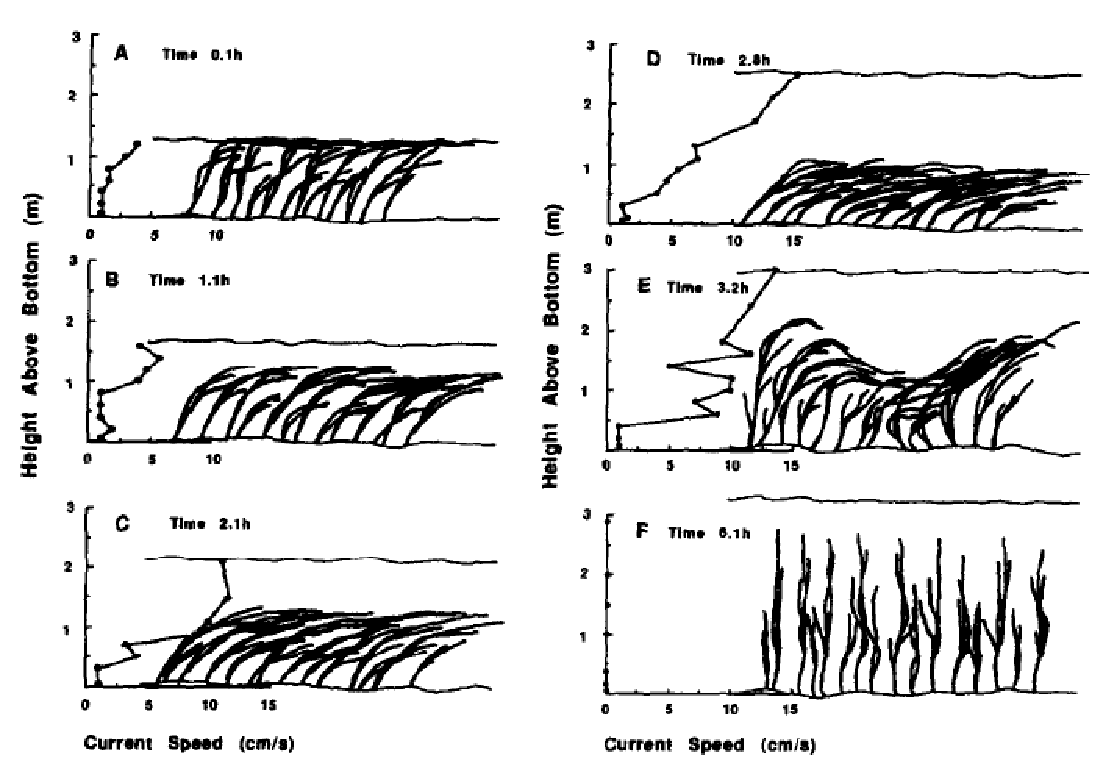
\includegraphics[scale=0.72]{Grizzle}}
 \caption{Sketches made by Grizzle, et al. \citep{Grizzle96} from direct observations of eelgrass blades in the mouth of the Jordan river, ME, USA, in response to a tidal
 flow through half a tidal cycle. The horizontal velocity profile is also plotted with each of the sketches. The grass spontaneously starts to wave in frame E, when the flow 
 speed exceeds a threshold of 10-15 cm/s.}
 \label{GrizzleFig}
\end{figure}

The current explanation of \textit{Monami} is proposed by Ghisalberti and Nepf \cite{Ghisal02,Nepf00} which is inspired by the work of Raupach for the case of terrestrial canopies, which is based on Kelvin-Helmholtz (KH) instability of free shear flow.
According to this mechanism the essential role of vegetation is to exert drag on the flow slowing it down, and giving rise to velocity differential between the canopy and the region above it. This so called shear layer profile is then expected to be hydrodynamically unstable to KH instability and break down into coherent vortices. The flexibility of grass blades then merely aids in visualizing these vortices by deforming as they are advected past by the flow.
According to this shear layer model, the velocity profile of flow through vegetation can be approximated to a characteristic shear like profile - `` one where shear does not arise from the boundary condition'' e.g. $U(y) = \Delta U[1+\tanh(y/\delta)]$, in an approximately unbounded domain $-\infty < y< \infty$, using the shear layer thickness $\delta$ determined by fitting to the measured mean velocity profile (e.g. see \ref{basicflow} ), the frequency predicted by KH instability agrees well with the laboratories observations.

However, several aspects of existing theory remain unexplained. First, the assumption of instability of perturbation to shear layer through a mechanism of Kelvin-Helmholtz relies on absence of any interaction between the flow perturbation and drag, making shear layer a inconsistent theory. Second, classical free shear flow is known to be unstable for all the Reynolds number. On the contrary, a threshold flow speed is observed in the field for the grass to spontaneously wave \cite{Grizzle96}; below this threshold speed the grass bends steadily in response to steady current. This threshold speed corresponds to a  critical Reynolds number $\approx O(1000)$, based on turbulent viscosity. 

Another seemingly related analysis of shear instability and coherent structure in shallow flow adjacent to emergent vegetation has been carried out by \cite{White07}, where presence of vegetation imposes extra drag in addition to drag caused by bed friction. In their analysis they also assumed steady profile to be hyperbolic tangent and flow domain to be infinite. They also assumed symmetric the drag due to vegetation and bed friction. Since both the dominant component of flow velocity are in the same plane as bed, we expect both these component to experience similar drag due to vegetation. However for flow through submerged vegetation one of dominant component is perpendicular (vertical velocity in Figure \ref{GrizzleFig}) to the bed plane and hence experience negligible drag as compared to the other component which is in the plane (horizontal velocity in Figure \ref{GrizzleFig}).

These drawbacks of existing theory suggest that flow through vegetation requires further investigation for better understanding of phenomenon.
\subsection{Our Approach}
In this study, we developed a mathematical model for the linear stability incorporating presence of grass through a drag field in the momentum equation of fluid. Although monami is manifested in the motion of grass, the drag exerted by the vegetation on the flow is central to the hypothesized instability. A linear stability analysis of this model shows that a competition between destabilizing effect of shear and stabilizing effect of drag dissipation leads to a critical flow condition characterized by Reynolds number above which flow becomes unstable leading to \textit{Monami}. Our linear stability analysis predicts existence of two different modes of instability which we termed as mode-1 and mode-2. Mode-1 is found to be instability localized on the length scale of shear layer formed near the canopy top whereas Mode-2 is represent the flow instability on the scale of full water column. We found that mode-1 shares many of characteristics of Kelvin-Helmholtz instability such as instability on the scale of 
shear layer thickness but is found to have significant differences as well. The prediction of critical Reynolds number and waving frequency associated with \textit{Monami} is found to compare well the experimental observations. Results from our analysis can also be applicable to many other related scenario such as flow over coral reefs, permeable sediments, flow through urban environments and therefore is expected to have wider impact. 

%\lipsum[21-40]

\nocite{Lax1956,Cooley1965,Banach1924}

\clearpage{\pagestyle{empty}\cleardoublepage}

\chapter{Mathematical Model}
Given the range of length scales in the canopy (leaf thickness $<$ 1mm, leaf width $\sim$ 1cm, canopy height $\sim 1m$, vegetation patch $10^2-10^3 m$), a fully resolved direct numerical solution is challenging and unnecessary. We instead exploit this separation of length scale between the canopy scale and its microstructure, and resort to modeling the aquatic vegetation as a homogenized multiphase medium which occupies no volume but exert drag on the fluid flow.
Because the leaves are wide but thin , the volume fraction of vegetation is less than $10\%$ \cite{chandler96} in the densest of seagrass canopies, and dominant interaction with the surrounding water is by exerting a drag. Hence to leading order, we ignore the space occupied by the grass in the fluid mass and momentum balance. In our model vegetation is represented as a continuum field $h(x,t)$. 

%Further, lab scale experiments have shown that flow instability and resulting flow structure leading to monami are present even when the flexible grass is replaced with rigid dowels \cite{Ghisal02, Nepf06}. Therefore to develop essential mathematical model we assume grass to be rigid and oriented vertically (along y direction) on average. Since the flow structure leading to monami is dominantly 2 dimension, we assume a two dimensional model for simplicity of calculation. In our mathematical model vegetation is assumed to be sufficiently dense so that drag exerted by the grass can be modeled as a continuum field. 

Here we present methods for averaging the flow equations in presence of vegetation. Following Pedras $\&$ de Lemos \cite{Pedras00} we first average over a time interval $\tau$ which is longer than the vegetation scale velocity fluctuation time, then perform spatial averaging. Denoting 
overbar to represent time averaged properties and the angel brackets to denote spatial averaged properties, for any fluid property $\phi$ such as velocity, pressure etc.
  \[ \bar{\phi}(x,y,z,t) = \frac{1}{\tau} \int_{t}^{t+\tau} \phi  \, dt \hspace{1.cm}  \langle \bar{\phi}\rangle = \frac{1}{A} \int_{A} \bar{\phi}  \,dx \,dy \]
  \[\phi = \bar{\phi}+\phi^{'} \hspace{1.cm}  \bar{\phi} = \langle \bar{\phi} \rangle \ +\phi^{''} \]
 Upon performing temporal averaging of Navier-Stokes and fluid continuity equation we arrive the following equations for fluid continuity and momentum balance.
 \begin{equation}
 \begin{split}
 \frac{\partial \bar{u_i} }{\partial x_i} &=0 \\
 \rho \left[ \frac{\partial  \overline{u_i}  }{\partial t}+  \overline{u_j}  \frac{\partial  \overline{u_i} }{\partial x_j} \right ] &= -\frac{\partial  \bar{p}   }{\partial x_i} + \mu \frac{\partial^2  \overline{u_i}  }{\partial x_j^2} - \rho \frac{\partial  \overline { u_i^{'} u_j^{'} }  }{\partial x_j} 
 \end{split}
 \end{equation}
 and further spatial averaging gives
  \begin{equation}\label{averaged_eq}
  \begin{split}
  \frac{\partial \langle \bar{u_i} \rangle}{\partial x_i}&=0 \\
 \rho \left[ \frac{\partial \langle \overline{u_i} \rangle }{\partial t}+ \langle \overline{u_j} \rangle \frac{\partial \langle \bar{u_i} \rangle}{\partial x_j} \right ] &= -\frac{\partial \langle \bar{p} \rangle  }{\partial x_i} + \mu \frac{\partial^2 \langle \bar{u_i} \rangle }{\partial         x_j^2} + \frac{\partial \langle \bar{\tau_{ij}} \rangle }{\partial x_j} -D_i
 \end{split}
 \end{equation}
 where $\rho$ is fluid density, $\mu$ is molecular viscosity and 
 $\tau_{ij}=-\rho \langle \overline{u_i^{'} u_j^{'}} \rangle  -\rho \langle{ \overline{u_i}^{''} \overline{u_j}^{''} } \rangle  $ is macroscopic shear stress tensor, which consists of Reynolds stresses ($ -\rho \langle \overline {u_i^{'} u_j^{'}} \rangle $) due to temporal fluctuation and dispersive stresses ($ -\rho \langle{ \overline{u_i}^{''} \overline{u_j}^{''} } \rangle $) due to spatial fluctuation. The drag force $D_i(x,y) = \langle \frac{\partial \overline{p}^{''}}{\partial x_i} \rangle - \langle \mu \frac{\partial^2 \bar{u_i}^{''} }{\partial x_j^2} \rangle $ is resistance due to vegetation, the sum of form and viscous drag over the averaging scale, which is zero above the vegetation i.e.  when $y>h(x,t)$. 
 %\begin{equation}
 % D_i = \langle \frac{\partial \overline{p}^{''}}{\partial x_i} \rangle - \langle \mu \frac{\partial^2 \bar{u_i}^{''} }{\partial x_j^2} \rangle
 %\end{equation}
 
 Since both dispersive stress ($-\rho \langle \bar{u_i}^{''} \bar{u_j}^{''} \rangle $)and molecular stress ($ \mu\ \del u_i / \del x_j $) are negligible compared to Reynolds stress ($-\rho \langle\bar{ u_i^{'} u_j^{'} } \rangle $), the equation \ref{averaged_eq} simplifies into
 \begin{equation}\label{averaged_eq2}
  \begin{split}
  \frac{\partial \langle \bar{u_i} \rangle}{\partial x_i}&=0 \\
 \rho \left[ \frac{\partial \langle \overline{u_i} \rangle }{\partial t}+ \langle \overline{u_j} \rangle \frac{\partial \langle \bar{u_i} \rangle}{\partial x_j} \right ] &= -\frac{\partial \langle \bar{p} \rangle  }{\partial x_i} -\rho \frac{\partial \langle \bar{u_i^{'}u_j^{'}} \rangle }{\partial x_j} -D_i
 \end{split}
\end{equation}
We further hypothesized that Reynolds stress can be estimated by using a constant eddy viscosity i.e. 
\[ -\rho \langle u_i^{'} u_j^{'} \rangle = \mu \left(\frac{\del \bar{u_i} }{\del x_j} + \frac{\del \bar {u_j} }{\del x_i}  \right)\]
From now-onwards $\mu$ stands for eddy viscosity rather than molecular viscosity, with this simplification equation \ref{averaged_eq} further simplifies into
 \begin{equation}\label{averaged_eq3}
  \begin{split}
  \frac{\partial \langle \bar{u_i} \rangle}{\partial x_i}&=0 \\
 \rho \left[ \frac{\partial \langle \overline{u_i} \rangle }{\partial t}+ \langle \overline{u_j} \rangle \frac{\partial \langle \bar{u_i} \rangle}{\partial x_j} \right ] &= -\frac{\partial \langle \bar{p} \rangle  }{\partial x_i} +\mu \frac{\partial^2 \langle \bar{u_i} \rangle }{\partial x_j^2} - D_i
 %\rho C_N d N_g \langle \overline{u_i}\rangle |\langle \overline{u_i} \rangle|
 \end{split}
\end{equation}
Which is same as Navier-Stokes equation with molecular viscosity replaced by a constant eddy viscosity, from now-onwards we will drop angle bracket and over bar 
for notational simplicity.
\begin{equation}\label{averaged_eq}
\begin{split}
  \grad .{\bu}&=0 \\
 \rho \left[ \frac{\partial {\bu}  }{\partial t}+  {\bu} . \grad \bu  \right ] &= - \grad{p}  +\mu \grad^2\bu - \mathbf{D}
\end{split}
\end{equation}
When the Reynolds number of the flow on the microstructure and molecular viscosity is small, the drag force $\mathbf{D}$ can be modeled according to Darcy's law $\mathbf{D} \propto \bu$. While there is no generic way to model the drag force when Reynolds number on microstructure is large ( O(100-1000) ), general principal of high-Reynolds number flows guide us towards a phenomenological model for drag. Firstly in this range of Reynolds number, the flow separate from grass blade forming a wake , and therefore it is reasonable to expect the drag to scale with dynamic pressure $\rho \bu_r^2$, where $\bu_r$ is the relative velocity between the fluid and the grass blade. Moreover, we assume that the drag is anisotropic; flow across the grass blade experiences more drag than the flow along the glass blade. Mathematically, the drag law uses projection of relative velocity along the blade and normal to the blade as.
\begin{equation}
 \bu_N = \bu_r.\bn,\hspace{0.5cm} \bu_T = \bu_r.\bt,\hspace{.5cm} \mathbf{D} = -\rho d(x,y)\left( C_N \bu_N |\bu_N|\bn + C_T \bu_T |\bu_T| \bt \right)
\end{equation} 
where $C_N$ and $C_T$ are drag coefficient in the normal and tangential directions respectively, $N_g$ is the grass number density, $d(x,y)$ is average grass diameter at location specified by co-ordinates $(x,y)$, $\bt$ is average unit vector tangent to the grass element at $(x,y)$ and $\bn$ is average unit vector normal to the grass blade at $(x,y)$. The orientation of grass blade can be obtained by solving force and torque balance equation together with a constitutive relation relating bending moment $M$ to the curvature $\kappa$
\begin{figure}
 \centerline{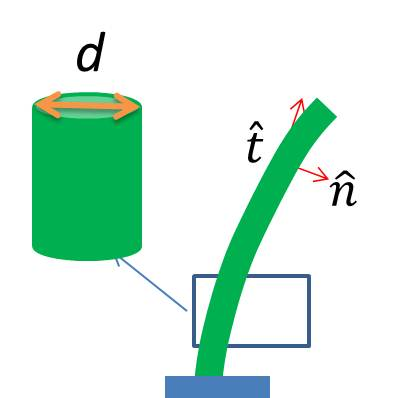
\includegraphics[width=2.8cm, height = 2.8cm]{Grass_mod1}\hspace{2.5cm} 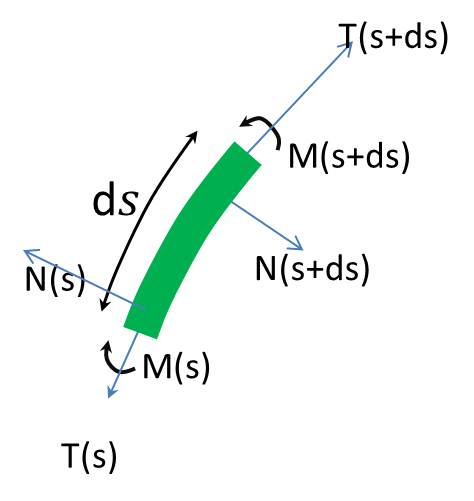
\includegraphics[width=3.cm,height=3.cm]{Grass_mod2}}
 \caption{Schematic of mechanics of individual grass blade deformation}
 \label{grass_blade_deformation}
\end{figure}
\begin{equation}
 \frac{\partial}{\partial s}\left( T\bt + N\bn \right)+\mathbf{f_d}+\mathbf{f_{buoy}} =0 \hspace{.5cm} \frac{\partial M}{\partial s} -N =0 \hspace{.5cm}  M = B\kappa
\end{equation}
Where $s$ is the arc-length along the grass blade, $\mathbf{f_{buoy}}$ is the force of buoyancy on the submerged grass blade and $\mathbf{f_{d}}$ is the drag force per unit length experienced by the grass blade. Since the marine grass blades are extremely flexible so we can safely ignore the role of bending stiffness in determining the orientation of grass blade,  which results in solving a simplified equation, subject to inextensiblity of the grass blades. 
\begin{equation}
  \frac{\partial}{\partial s} T\bt +\mathbf{f_d}+\mathbf{f_{buoy}} =0
  \label{orientation_eq}
\end{equation}
The equation \eqref{orientation_eq} together with the equation \eqref{averaged_eq} can be solved subject to appropriate boundary condition to predict flow structure and grass orientation.

Although {\monami} is manifested in the motion of grass, the drag exerted by the vegetation on the flow is central to flow instability leading to {\monami}. Since the instability and resulting flow structures leading to monami persist even when the flexible grass mimics are replaced with the rigid dowels \cite{Ghisal02,Nepf06}. Therefore, to develop essential mathematical model, we assume grass blade to be rigid on average oriented vertically.
Boundary condition for \eqref{averaged_eq} on the bed include no-shear, and a specified number density of grass. The no shear condition arises because, for dense vegetation the shear stress exerted by the bottom surface is expected to be negligible compared to the vegetation drag. On the top surface, a rigid-lid condition (no shear and no normal velocity) or a free surface condition is suitable. In this analysis we have used rigid-lid condition on the top surface. The prediction of mean velocity made based on these condition agrees well with the experiments (e.g see Figure \ref{basicflow} ). 
%\lipsum[61-80]

\clearpage{\pagestyle{empty}\cleardoublepage}
\chapter{Linear stability analysis}
The usual response of submerged grass to steady current is to remain bend in some fixed configration. However above certain flow velocity the grass beds shows coherent large amplitude oscillation as well, such response of time dependent large amplitude oscillation exhibited by sea grass under the influence of otherwise steady steady current is thought to be understood as result of hydrodynamic instability. In order to understand nature of the flow instability associated with monami, we first calculate the fully developed steady solution $\bu = U(y)\boldsymbol{\hat{x}}$ of ~\eqref{averaged_eq3} driven by constant pressure gradient $dP/dx$, and use it to non-dimensionlize the mathematical model. The momentum balance \eqref{averaged_eq3} for $U(y)$ simplifies to
\begin{equation}
\begin{split}
 -&\frac{dP}{dx}+\mu U''(y) -S(y) \rho C_N d N_gU |U| =0\\
 &S(y) = 1, \hspace{2cm} 0<y<\hg\\
 &S(y) = 0, \hspace{2cm} \hg< y< 2H
\label{base_equ}
\end{split}
\end{equation}
Eq. \eqref{base_equ} is solved subject to no shear at the boundaries, i.e., $U'(0) = U'(2H) = 0$. In real flow the true boundary condition at the bottom is no slip velocity, however the boundary layer formed due to no slip condition is so thin ($\approx 0.5 cm$) that it's hardly visible in experiments as can be seen from the experimental data of \ref{Nepf04} in Figure \ref{basicflow}. Due to presence of dense vegetation the shear stress exerted by the bottom surface is expected to be negligible compared to the vegetation drag \cite{Nepf04 } and hence the bottom boundary condition can be approximated by no shear $U'(0)=0$ condition.
On the top surface, a rigid lid condition ( no shear and no normal velocity ) or free surface is suitable. Since changes in water surface elevation due to presence of \monami  is small compared to the depth of water channel, we can approximate the top surface by no shear condition ($ U'(2H)=0$ ) as well.
A comparison of the steady flow profile from the solution of ~\eqref{base_equ} with experimental measurements is shown in Fig \ref{basicflow}.
\begin{figure}
\centerline{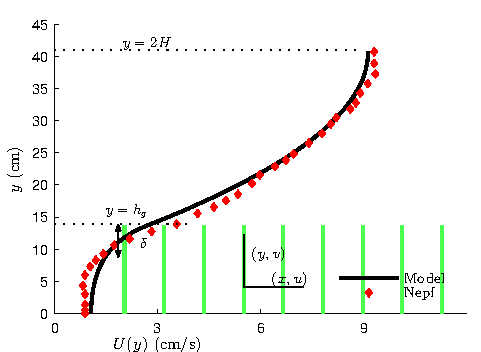
\includegraphics[scale=.99]{Grass_Base_Nepf} }
% 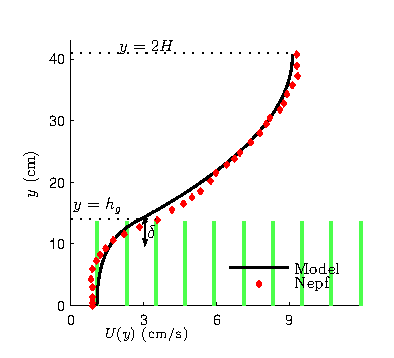
\includegraphics[width=15cm]{Grass_Base_Nepf_shear}
\caption{
Schematic setup and comparison of our steady flow profile with that from the experiments in ref. \cite{Nepf04} (Case I from Table 1) %  with 1250 plants/m$^2$, plant height = 13.7$\pm 0.2$ cm and blade width of 0.64 cm)
 and its approximation with $U_0=7.28$ cm/s and $\delta = 5.02$ cm in our model. The grass extends up to $y=\hg$ in the water column of depth $2H$. 
The steady velocity profile can be decomposed into a parabolic profile in the unvegetated region, a uniform profile deep within the vegetation, and a boundary layer of thickness $\delta$ near the grass top. 
The dependence of the boundary layer thickness (estimated as $|U/U_y|$ at $y=\hg$ from the numerical solution of \eqref{base_equ}) on the vegetation density parameter $\ReyNdg$ is shown in the inset.
}
\label{basicflow}
\end{figure}
The profile $U(y)$ has three distinct regions.
Within the vegetation, it is approximately uniform with $ U(y) \approx U_g = \sqrt{\frac{-dP/dx}{\rho C_N dN_g}}$ which arise from the balance of the drag with the pressure gradient. 
Outside the vegetation, the velocity has a simple parabolic profile similar to a Poissueille profile, arising from the balance between pressure and viscous forces together with the free shear condition at the top surface. 
At the grass top, continuity of shear stresses results in a boundary layer of thickness $\delta$ - `` one where shear does not arise from boundary conditions''. Denoting $\ubl$ to be the velocity scale in the boundary layer, and $U_0 = {(-dP/dx)~H^2}/{\mu}$ the velocity scale in the unvegetated region, the balance between viscous forces and vegetation drag with in grass implies $(\mu \ubl/\delta^2 \sim \rho C_N d N_g \ubl^2)$, and the continuity of shear stress across the grass top implies $(\ubl/\delta \sim U_0/H)$.
Solving for $\delta$ and $\ubl$ yields $\delta/H \sim \ubl/U_0 \sim (\Rey \Ndg )^{-1/3}$, %where $\Ndg = \left(C_N d H N_g\right)$ is the vegetation frontal area per bed area, and $\Rey=\rho U_0 H/\mu$ is the Reynolds number of the flow. 
A numerical estimate of $\delta$ (estimated as $U/U_y$ at $y=\hg$) is compared with this prediction in Fig. \ref{basicflow} (inset).
We identify the boundary layer to be analogous to the shear layer \cite{Ghisal02,Nepf04} in the previous explanation of \monami.
The dependence of $\delta$ on $N_g$ gives us a way to systematically investigate the effect of the shear layer thickness on the instability mechanism.
Fig. \ref{basicflow} also shows that the asymptotic regime of a thin boundary layer is expected to hold for $\ReyNdg \gtrsim 100$. 
In this notation, $U_g/U_0 = (\Rey \Ndg)^{-1/2}$ (used later in deriving \eqref{eqn:mode2asymp}). 
\begin{figure}
\centerline{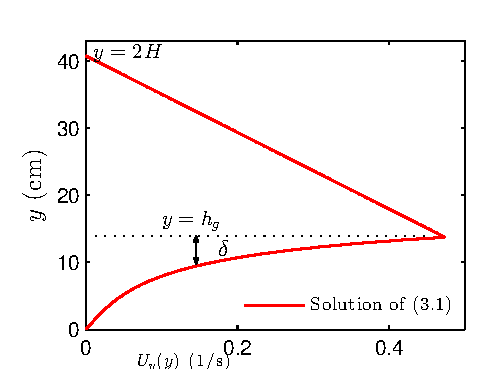
\includegraphics[scale=1.]{Grass_Base_Nepf_shear_scale} 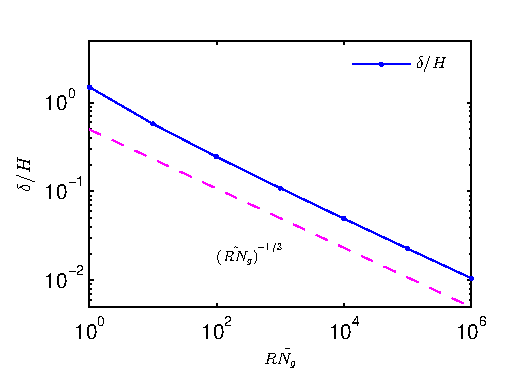
\includegraphics[scale=1.]{Grass_shear_scale}}
% 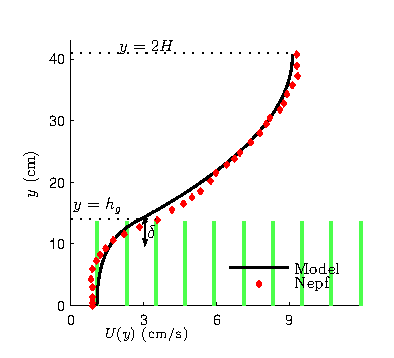
\includegraphics[width=15cm]{Grass_Base_Nepf_shear}
\caption{
Schematic setup and comparison of our steady flow profile with that from the experiments in ref. \cite{Nepf04} (Case I from Table 1) %  with 1250 plants/m$^2$, plant height = 13.7$\pm 0.2$ cm and blade width of 0.64 cm)
  from the numerical solution of \eqref{base_equ}) on the vegetation density parameter $\ReyNdg$ is shown in the inset.
}
\end{figure}
\begin{figure}
\centerline{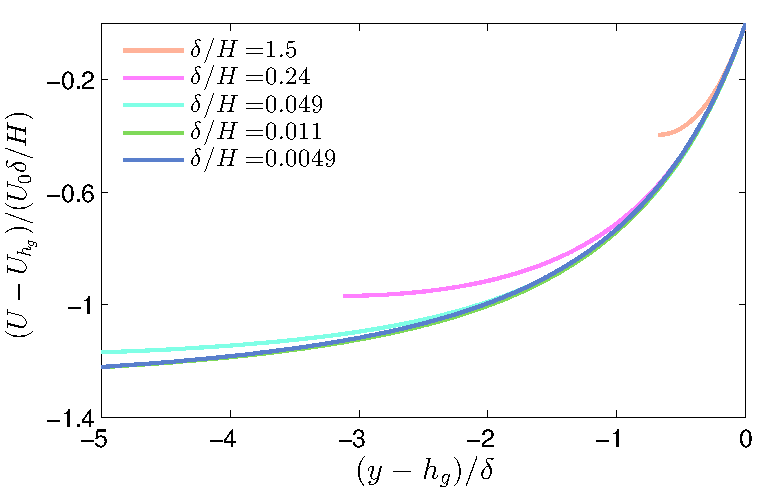
\includegraphics[]{Grass_shear_scale_collapse} }
% 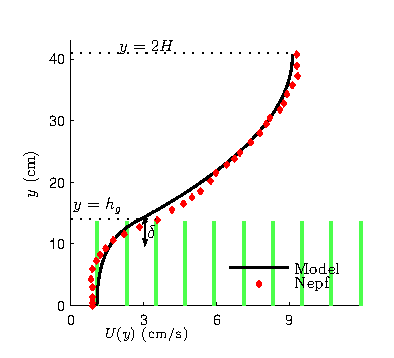
\includegraphics[width=15cm]{Grass_Base_Nepf_shear}
\caption{
Schematic setup and comparison of our steady flow profile with that from the experiments in ref. \cite{Nepf04} (Case I from Table 1) %  with 1250 plants/m$^2$, plant height = 13.7$\pm 0.2$ cm and blade width of 0.64 cm)
  from the numerical solution of \eqref{base_equ}) on the vegetation density parameter $\ReyNdg$ is shown in the inset.
}
\end{figure}

Next we substitute $\bu = (U+\tilde{u}, \tilde{v})$, $p=P+\tilde{p}$ in ~\eqref{navier-stokes} and expand to linear order to investigate the evolution of small perturbations $(\tilde{u}, \tilde{v})$, which obey
\begin{equation}
\begin{split}
\rho(u_t+U u_x+vU_y) &= -p_x+ {\mu}\nabla^2u-2S\rho C_{N}dN_{g}Uu, \\
\rho(v_t+ Uv_x) &= -p_y+ {\mu}\nabla^2v, \hspace{0.3cm} \nabla\cdot\bu=0,
\label{LinearizedNavierStokes}
\end{split} 
\end{equation}
where the tilde are dropped.
These equations are non-dimensionalized using half channel height $H$, velocity $U_0$, and time $H/U_0$, leading to three non-dimensional parameters, \textit{viz.} $\Rey$, $\Ndg$, and the vegetation submergence ratio $\hg/H$. 
We also use $\delta/H$ in lieu of $\Ndg$ to parametrize the vegetation density and help elucidate the instability mechanism. 
Using a stream function $\psi$ with $u = \psi_{y}, v= -\psi_x$ to satisfy mass balance, we seek a solution of 
the form $\left(u,v,\psi \right)= \left(\hat u(y), \hat v(y), \phi(y) \right)e^{ikx+\sigma t}$ to obtain a modified Orr-Sommerfeld equation \cite{Drazin81,Chen97,Chu91} 
\begin{equation}
\begin{split}
\Rey^{-1}\left(D^2 -k^{2} \right)^2\phi &= \left[ \left({\sigma}+ikU\right) \left(D^2-k^2\right) -ikU_{yy}\right]\phi + \Ndg D\left(2 S U D \phi\right),
\label{Orr-somerfield}
\end{split}
\end{equation}
where $D=d/dy$, and subject to the boundary conditions $\phi = D^2\phi = 0$ at $y=0$ and $y=2$. 
The growth rate $\sigma$ for a given wave number $k$ appears as an eigenvalue that allows a non-trivial solution $\phi$ of  \eqref{Orr-somerfield}.
\section{Numerical Method}
  In order to solve \eqref{Orr-somerfield}, we used finite difference with $N$ equally spaced grid points $(y_i = i\Delta y, \Delta y = \frac{2}{N})$, and used second order approximation for various terms in \eqref{Orr-somerfield} at these grid points. We used following approximation for evaluating various derivatives appearing in \eqref{Orr-somerfield}
  \begin{equation}
  \begin{align}
    \left.{ D^4\phi} \right|_i &= \frac{ \phi_{i+2}-4\phi_{i+1}+6\phi_{i}-4\phi_{i-1}+\phi_{i-2} }{\Delta y^4} - \frac{\Delta y^2}{6} \left. \frac{\del^6 \phi}{\del y^6} \right |_i \\
    \left. D^2\phi \right|_i &=  \frac{\phi_{i+1} -2\phi_i +\phi_{i-1}}{\Delta y^2} - \left. \frac{\Delta y^2}{12} \frac{\del^4 \phi}{\del x^4} \right|_i \\    
    \left. D\phi \right|_i &=  \frac{\phi_{i+1} -\phi_{i-1}}{2\Delta y} - \left. \frac{\Delta y^2}{6} \frac{\del^3 \phi}{\del x^3} \right|_i \\
    \end{align}
  \end{equation}
The boundary conditions at the top and bottom surface are approximated by $\phi_0 = 0$,  $\phi_{N+1} = 0$ to satisfy $\phi=0$ at the top and bottom surface.
The zero shear condition at the top and bottom surface ($D^2\phi=0$) are expressed by $\phi_{-1} = -\phi{1}$ and $\phi_{N+1} = -\phi_{N}$. The last term in \eqref{Orr-somerfield} give rise to a dirac-delta term $2\Ndg U_g D\phi_g \delta(y-h_g)$, where $U_g$ is velocity the grass tip and $\phi_g$ is value of $\phi$ at the grass tip. We approximate the term with dirac-delta as $2\Ndg U_g D\phi_{g} \frac{1}{\Delta x}$.
The base velocity profile at these grid points are evaluated by solving \eqref{base_equ}. Using these approximation we can rearrange terms in \eqref{Orr-somerfield} 
\begin{equation}
\begin{split}
A\phi &= \sigma B \phi\\
A &= \Rey^{-1}\left(D^2 -k^{2} \right)^2\phi-ikU \left(D^2-k^2\right)\phi + ik U_{yy}\phi -\Ndg D\left(2 S U D \phi\right)\\
%\Rey^{-1}\left(D^2 -k^{2} \right)^2\phi-ikU \left(D^2-k^2\right)\phi +5 ik U_{yy}\phi &-\Ndg D\left(2 S U D \phi\right)  =\\
B &= {\sigma} \left(D^2-k^2\right) \phi
\end{split}
\end{equation}
where the operator $A$ and $B$ are approximated at the grid points using finite difference method. This results in solving finite dimensional generalized eigen-value problem, whose solution provide growth rate $\sigma$ and eigen mode $\phi$ for a perturbation of wavenumber $k$ to the base velocity profile $U(y)$.  
\begin{figure}
 \centerline{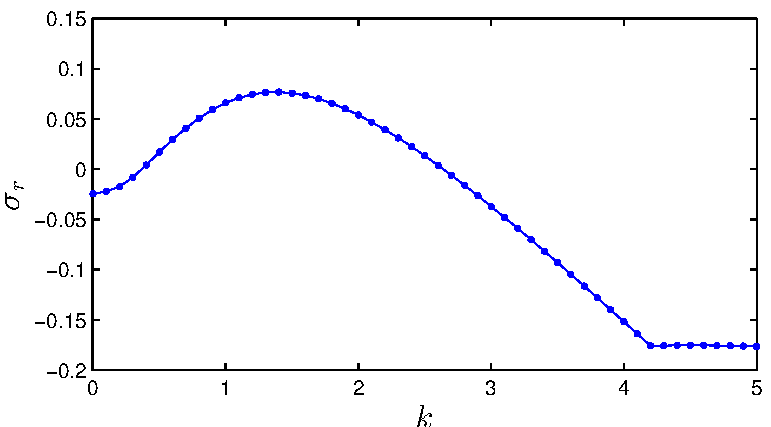
\includegraphics{GrowthrateVsK}}
 \caption{Growth rate of perturbation ($\sigma_r$) to solution of \eqref{base_equ} as predicted by the solution of \eqref{Orr-somerfield}. The  Reynolds number, grass number density and submergence ratios are $R=500$, $\Ndg=2$ and $h_{grass}/(2H) = 0.4$ respectively }
\end{figure}


%\lipsum[81-100]

\begin{figure}
  \centering
  \begin{tikzpicture}[scale=3]

  \draw [fill=red!20!white] (1,1) -- ++(0,-2) -- ++(-2,0) -- ++(0,2) -- cycle;
  \draw [fill=blue!20!white,opacity=0.4] (0,0) circle(2cm);
  \node [font={\Large\sf}] (yo) at (0,0) {Yo, yo, home slice};
  \draw[->,very thick, dashed] (yo) to [out=45,in=-45] (3,0);

\end{tikzpicture}

  \caption[Awesome picture]{Isn't this picture awesome?}
\end{figure}

\begin{figure}
  \centering
  \begin{tikzpicture}
  \draw [fill=red!70!white,circular drop shadow={shadow scale=1.05},very
  thick,rotate=45,opacity=0.7] (0,0) rectangle (3,2);


  \draw [fill=blue!70!white,circular drop shadow={shadow scale=1.05},very
  thick,rotate=135,opacity=0.7] (0,0) rectangle (3,2);
  \draw [fill=orange!70!white,circular drop shadow={shadow scale=1.05},very
  thick,rotate=225,opacity=0.7] (0,0) rectangle (3,2);
  \draw [fill=green!70!white,circular drop shadow={shadow scale=1.05},very
  thick,rotate=-45,opacity=0.7] (0,0) rectangle (3,2);
\end{tikzpicture}

  \caption[Tubular picture]{Totally tubular, dude}
\end{figure}

\clearpage{\pagestyle{empty}\cleardoublepage}

\chapter{Results}
\subsection{Unstable modes and critical parameters}
\begin{figure}
\begin{center}
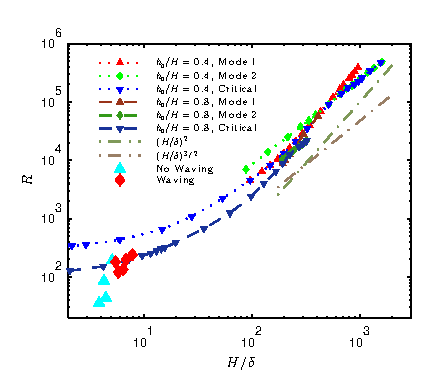
\includegraphics[scale = 0.95]{new_graph_R_vs_delta}\\
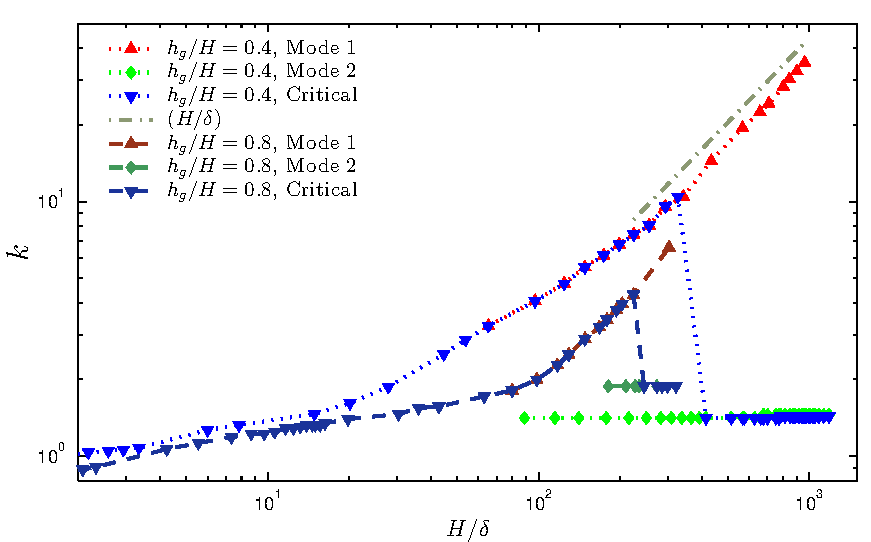
\includegraphics[scale = 0.95]{new_graph_K_vs_delta}
% 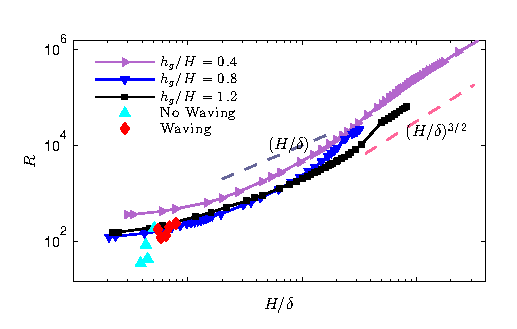
\includegraphics[width=12cm]{Critical_Re_vs_delta_noshear} \\
% \vspace{-6mm} \hspace{-5mm}
% 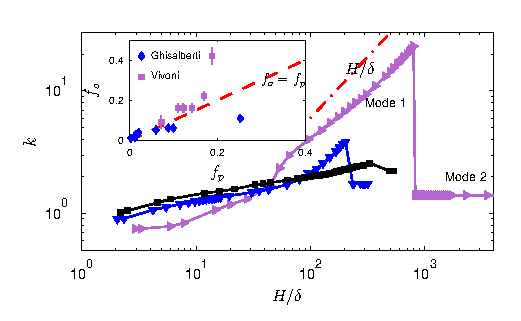
\includegraphics[width=12cm]{K_vs_shear_width_noshear}
\end{center}
\caption{
Critical Reynolds number, threshold Reynolds number for Mode 1 and Mode 2 (left) and the corresponding marginally stable wave number (right) for different submergence ratio as a function of vegetation density parametrized by the boundary layer thickness. 
Parameters from experiments reported by \cite{Ghisal02} to exhibit or suppress synchronous waving are also included in the left panel. 
In order to estimate the $\Rey$ for these experiments, a representative value of $\mu=0.1$ Pa~s was assumed.
}
\label{Re_vs_delta}
\end{figure}
In order to understand Critical criteria for waving we solve \eqref{Orr-somerfield} numerically for $\sigma$ and $\phi$. A threshold in $\Rey$, above which the flow is unstable (Re$(\sigma)>0$) for at least one $k$, emerges from the solution of ~\eqref{Orr-somerfield}. 
The dependence of this threshold $\Rey$, and the corresponding marginally stable wavenumber $k$, on $\delta/H$ and $\hg/H$ is shown in Fig.~\ref{Re_vs_delta}, and is found to compare well with experimental observations of \cite{Ghisal02}.
The threshold $\Rey$ increases with the vegetation density, indicating a competition between the destabilizing shear in the flow, and the stabilizing effect of damping due to vegetation drag.
% A similar conclusion was presented for an analogous problem (flow around an emergent (i.e., $\hg>2H$) sea grass patch), but by assuming $U(y)$ to be a tanh-profile, and neglecting the viscous term \citep{White07}.
%Previous calculations for terrestrial grass either exclude the vegetation drag in their models \cite{Raupach96}, or assume the mean velocity profile \textit{ad hoc} \citep{Raupach96,Delangre06}.
%A threshold flow condition is not reported previously either for terrestrial or submerged marine meadows.
The frequency (Im$(\sigma)$) of the fastest growing mode also agrees well with observed behavior -- frequency of \monami, maxima in the velocity spectra, and frequency of vortex passage in lab scale experiments \cite{Ghisal02} -- for cases where the vegetation was sufficiently dense to be modeled by a continuum drag field as shown in Fig.~\ref{frequency_comparison}. For completeness, the comparison of solution of \eqref{base_equ}
with the velocity profile observed in the lab scale experiment of \cite{Vivoni98} are shown in \ref{VivoniFig}. The velocity profile for experiments of \cite{Ghisal02} are not
available. The calculated velocity profiles for both these experiments are estimated using the constrain of given flow rate, grass number density and the submergence ratio. The experimentally observed \monami ~wavelengths are not available for comparison.
\begin{figure*}
 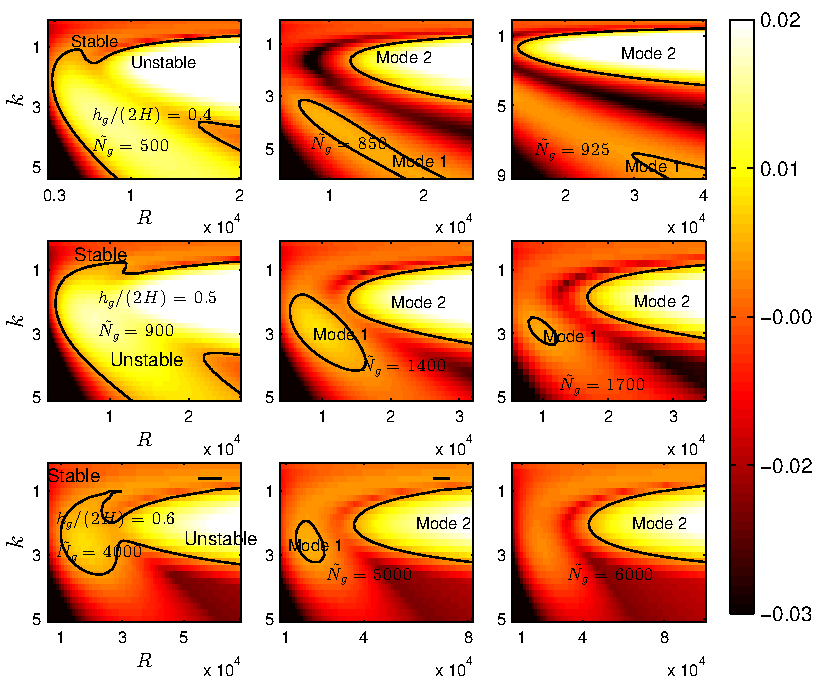
\includegraphics[width=\textwidth]{SetAll_imgsc3}
%\end{figure}
%\begin{figure*}
%\begin{tabular}{cccc}
%{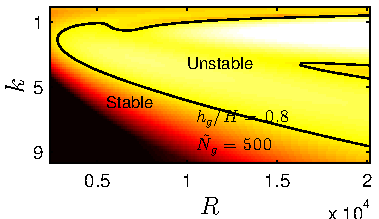
\includegraphics[height = 4cm, width = 5.8cm]{Set4_dens28_imgsc}} &
%{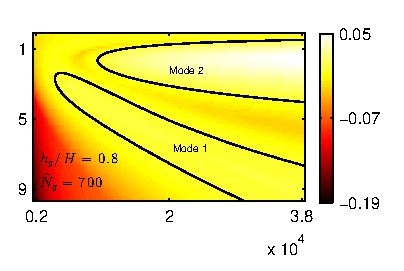
\includegraphics[scale = 0.67]{Set4_dens30_imgsc}} &
%{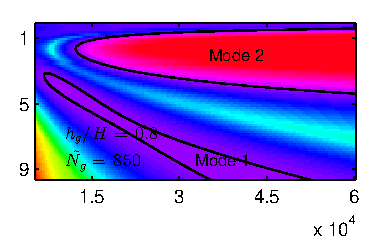
\includegraphics[height = 4cm,width = 5.8cm]{Set4_dens32_imgsc}} &
%{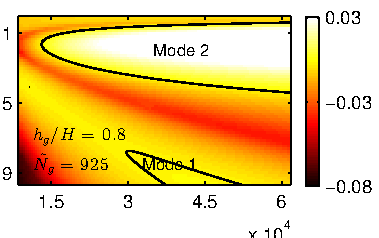
\includegraphics[height = 4.15cm,width=6.5cm]{Set4_dens34_imgsc}} \\
%{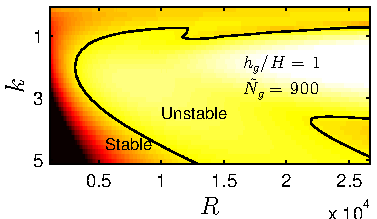
\includegraphics[height = 4cm, width = 5.8cm]{Set5_dens38_imgsc}} &
%{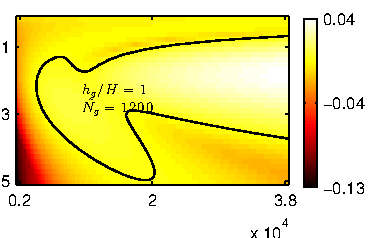
\includegraphics[scale = 0.67]{Set5_dens40_imgsc}} &
%{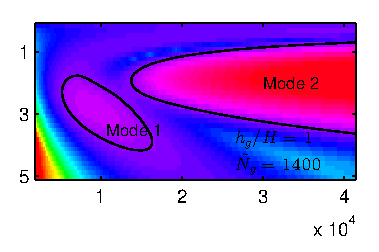
\includegraphics[height = 4cm, width = 5.8cm]{Set5_dens42_imgsc}} &
%{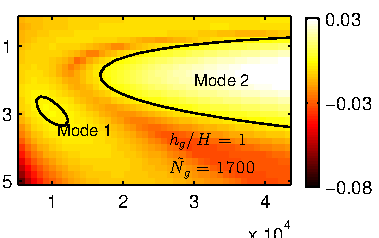
\includegraphics[height = 4.15cm,width=6.5cm]{Set5_dens46_imgsc}} \\

%{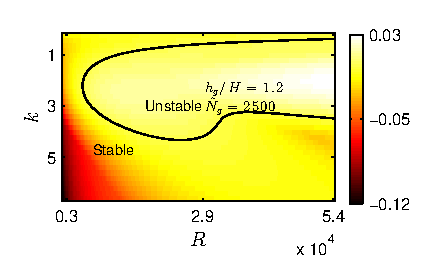
\includegraphics[scale = 0.67]{Set6_dens32_imgsc}} &
%{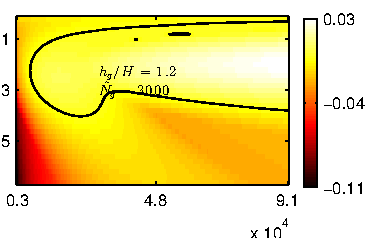
\includegraphics[scale = 0.67]{Set6_dens34_imgsc}} &
%{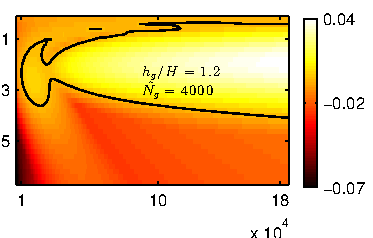
\includegraphics[scale = 0.67]{Set6_dens36_imgsc}} &
%{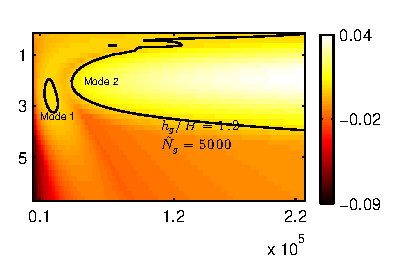
\includegraphics[scale = 0.67]{Set6_dens38_imgsc}}
%\end{tabular}
\caption{
$\text{Re}(\sigma)$ and the neutral curve ($\text{Re}(\sigma)$=0) as a function of wavenumber and $\Rey$ for parameters shown in the corresponding panel.  
As $\Ndg$ increases, the unstable region splits into two labeled as ``Mode 1'' and ``Mode 2''. 
For $\Ndg$ below (above) a critical value, Mode 1 (Mode 2) sets the threshold $\Rey$.
}
\label{K_Re_sigma_set3}
\end{figure*}
To better understand the instability mechanism, we consider the dependence of the fastest growing wavenumber on $\delta$.
The fastest growing wavenumber first increases proportional to $H/\delta$, but at a critical $\delta$ discontinuously jumps and remains $O(1)$ (see Fig.~\ref{Re_vs_delta}). 
To aid in explaining this behavior, we show heat maps of Re$(\sigma)$ as a function of $\Rey$ and $k$, for different $\hg/H$ and $\Ndg$ in Fig.~\ref{K_Re_sigma_set3}. 
The smallest $\Rey$ on the neutral curve (Re$(\sigma)=0$) sets the threshold. 
We observe that as $\Ndg$ increases, the unstable region splits into two; we refer to the region with the higher $k$ as ``Mode 1'', and the one with the lower $k$ as ``Mode 2''. 
For $\hg/H\lesssim 0.9$, the unstable region for Mode 1 recedes to higher $\Rey$, and for $\hg/H \gtrsim 0.9$, the region shrinks to zero size.
In either case, due to such behavior the most unstable mode transitions discontinuously from Mode 1 to Mode 2.
All experimental data we have found corresponds to a vegetation density for which the unstable region in the $\Rey-k$ space has not split into two. 
The distinct asymptotic behavior of the two modes as $\Ndg \gg 1$ distinguish them from each other and facilitate comparison with KH instability mechanism.

\subsection{Mode 1}
We numerically observe that the threshold Reynolds number for Mode 1 instability scales as  $\Rey \sim (H/\delta)^2$ (or $\Rey \propto {\Ndg}^{2}$). 
Our calculations also show that Mode 1 asymptotically localizes to the boundary layer near the grass top, and exhibits highest growth for a perturbation of  $k \sim H/\delta$ (see Fig.~\ref{Re_vs_delta}). 
The behavior of this critical Reynolds number can be understood by considering the limit $\Rey \gg 1$ and $\Ndg \gg 1$.
Estimating the size of various terms of ~\eqref{Orr-somerfield} within the boundary layer in this limit help us understand the behavior of the critical $\Rey$. 
Using $D\sim H/\delta$, $\sigma \sim O(1)$, and $U=\ubl \sim \delta/H$ in the boundary layer; the magnitude of the advection term is $ (H/\delta)^2$  (or $\Rey^{2/3} \Ndg^{2/3}$), and the viscous and vegetation drag terms are $(1/\Rey) (\delta/H)^{-4}$ (or $(\Rey^{1/3} \Ndg)^{4/3})$. 
The advection term, viscous term and vegetation drag terms balance when $\Rey \sim (H/\delta)^2$ (or $\Rey \sim {\Ndg}^{2}$).

\begin{figure}
\centerline{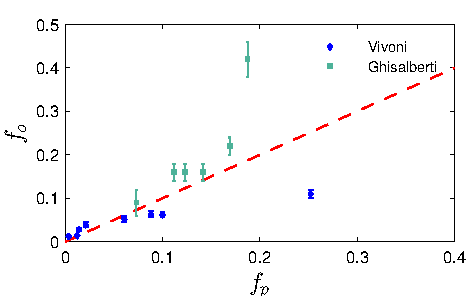
\includegraphics[]{new_graph_freq}}
\caption{Comparison of experimental observations of the experimentally measured dominant frequency $f_o$ (in Hz) with the predictions $f_p=\text{Im}(\sigma)$ from the solution of ~\eqref{Orr-somerfield}. 
The experimental data in the inset is obtained from \cite{Ghisal02} (Ghisalberti) and \cite{Vivoni98} (Vivoni). 
In order to estimate the $\Rey$ for these experiments, a representative value of $\mu=0.1$ Pa~s was assumed.
}
\label{frequency_comparison}
\end{figure}

\begin{figure}
 \centerline{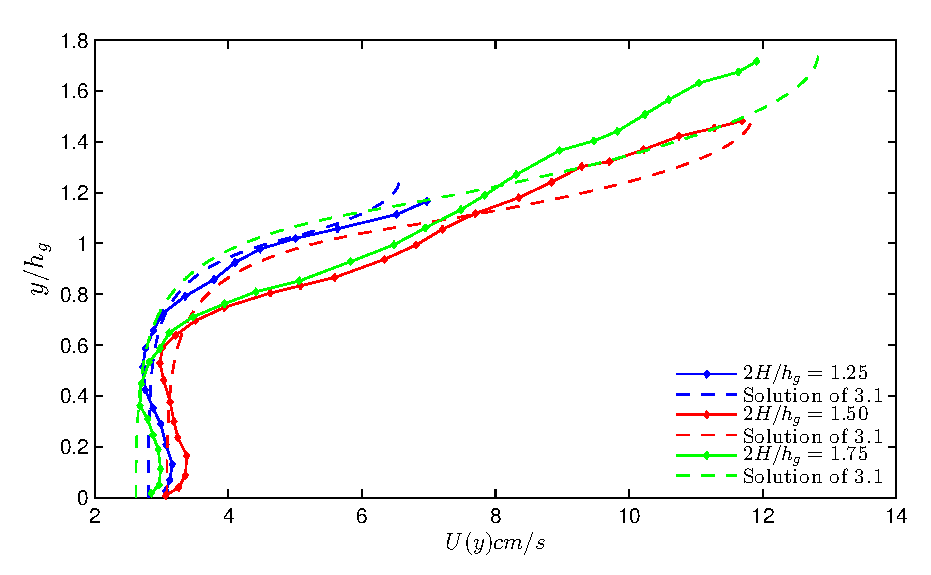
\includegraphics[]{Vivoni_Fig3_6_zero_shear_match} 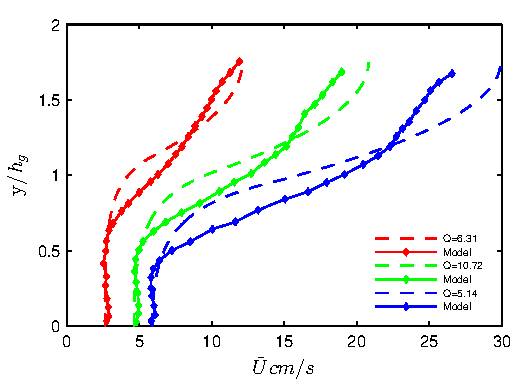
\includegraphics{Vivoni_Fig3_7_zero_shear_match}}
 \caption{Comparison of experimental velocity profile of lab scale experiments with the solution of \eqref{base_equ} for \textit{Case A } and \textit{Case B} experimental observation of \cite{Vivoni98} }
 \label{VivoniFig}
\end{figure}

To further understand the mechanism of Mode 1, we rescale \eqref{Orr-somerfield} near the grass-top using the the boundary layer scalings $\eta = y/(\delta/H)$, 
$U(y) = (\delta/H)\bar{U}(\eta)$ and $k = (H/\delta) \bar{k}$.
With these scalings ~\eqref{Orr-somerfield} simplifies to
\begin{equation}
\begin{split}
\left(\bar{D}^2 -\bar{k}^{2} \right)^2\phi &= (\Rey/\Ndg^2)^{1/3} \left[ \left({\sigma}+i\bar{k}\bar{U}\right) \left(\bar{D}^2-\bar{k}^2\right) -i\bar{k}\bar{U}_{\eta\eta}\right]\phi + \bar{D}\left(2S \bar{U} \bar{D} \phi\right),
\label{eqn:mode1asymp}
\end{split}
\end{equation}
in a region of thickness O($\delta$) near $y=\hg$, where $\bar{D} = d/d\eta$. 
Since $(\Rey/\Ndg^2)$ is the only remaining parameter in \eqref{eqn:mode1asymp}, the mode shape and solution are expected to converge in the limit $\Rey \gg 1$, $\Ndg \gg 1$, but $\Rey/\Ndg^2$ fixed.
Our numerical findings confirm this expectation; the critical $\Rey$ scales as $(H/\delta)^2$ as shown in Fig.~\ref{Re_vs_delta} and the mode shapes are self-similar with length scale $\delta$, as shown in Fig \ref{Asymptotic_mode}. 

Mode 1 shares many characteristics with the KH instability (see Table \ref{tab:comparison}). 
The fastest growing wavenumber at the critical $\Rey$ scales as $k \propto (H/\delta)$, similar to KH instability. 
The extent of the unstable mode is also localized to the boundary layer region.
The porous nature of the vegetation implies that a weak flow of magnitude $\ubl = U_0 \delta/H$ penetrates a thin boundary layer region $\delta$, and therefore the shear gradient $U_{yy} \sim U_0/\delta H$ is largest in this region. 
The strong shear gradient $U_{yy}$ in the boundary layer plays a central role in destabilizing the flow and localizing the instability to that region. 
Our detailed description of Mode 1, given by \eqref{eqn:mode1asymp} also highlights key differences with formulations of KH. 
KH is usually described using the inviscid Rayleigh's equation, 
\begin{align}
\left(\sigma+ikU\right) \left(D^2-k^2\right)\phi =  ikU_{yy}\phi, 
\label{eqn:Rayleigh}
\end{align}
and is therefore not parametrized by the Reynolds number.
Describing the instability using the Orr-Sommerfeld equation introduces the Reynolds number as a parameter, but shear flows with tanh-profiles are unstable for all values of the parameter {Drazin81}.
Therefore, based on the inviscid formulations of KH instability, the origin of the threshold flow conditions observed in experiments and the field is unclear.

In our model, (turbulent eddy) viscosity sets the scale of the boundary layer, and therefore for Mode 1.
However, the boundary layer is established only in the vegetated region; the velocity profile does not saturate on the scale of $\delta$ in the unvegetated region.
The threshold flow condition arises from a competition between the destabilizing role of fluid inertia, which is very similar to the one played in KH, and the vegetation drag.
The vegetation drag may not be neglected within this boundary layer, and therefore plays a central role in the Mode 1 instability mechanism.

%We expect identical asymptotic behavior for a fixed relative magnitude of the terms on the r.h.s. to those on the l.h.s. of \eqref{eqn:mode1asymp}, which is $(\Rey \delta/H)^{3/2}$ (or $\Rey/\Ndg^{1/2}$).
%Therefore the threshold obtained for Mode 1 is $\Rey \propto H/\delta$ (or $\Rey \propto \Ndg^{1/2}$) explaining the numerically observed asymptote (see Fig.~\ref{Re_vs_delta}). 
%This analysis also concludes that the mode structure is self-similar over the length scale $\delta$ for fixed $\Rey/\Ndg^{2}$; the verification of this idea is shown in Fig.~\ref{Asymptotic_mode} (inset).

\begin{figure}
\centerline{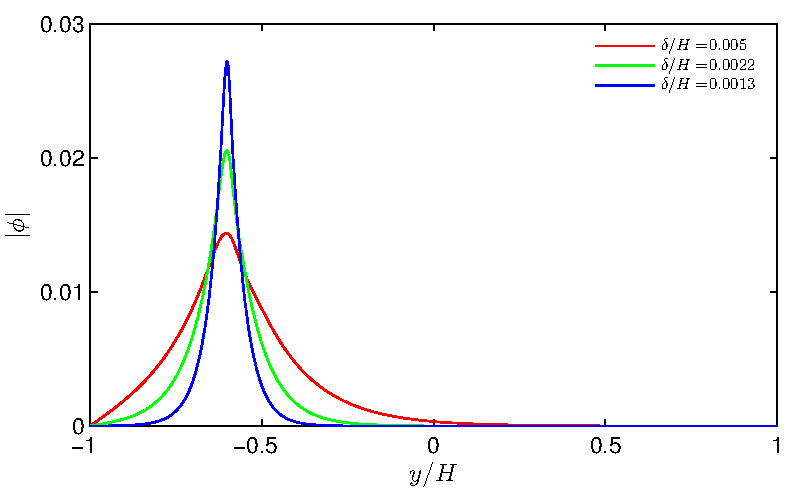
\includegraphics[scale=1.2]{Asymptotic_noshear}}
% 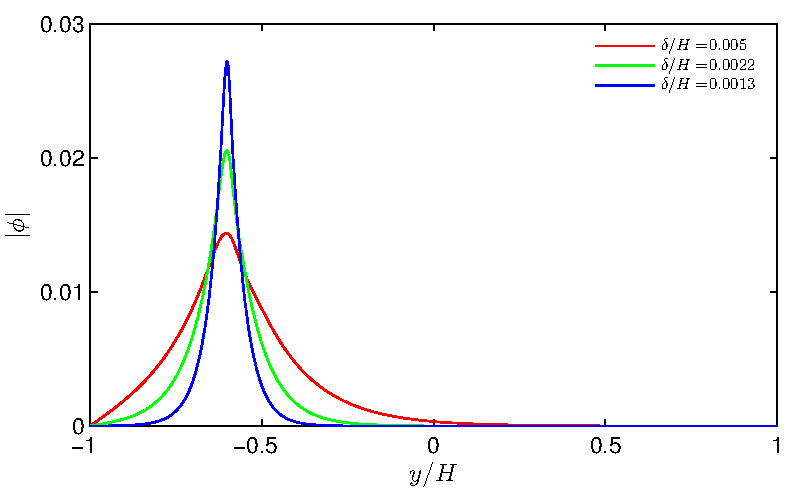
\includegraphics[width=12cm]{Asymptotic_noshear}
\caption{
Plot of the neutral Mode 1 (solid) and Mode 2 (dashed) shape $|\phi|$ in the limit of small $\delta/H$ for $\hg/H=0.2$. 
% Mode 1 is shown in solid and Mode 2 is shown in dashed. The parameters for Mode 2 shapes are chosen such that $\Rey \gg 1$, $\Ndg \gg 1$ (specified in terms of $\delta/H$) but $\Rey/\Ndg = O(1)$. 
The approach of mode shapes to each other for these small values of $\delta/H$ indicates that the dense vegetation asymptote is reached. 
Mode 1 shapes appear self-similar in shape as $\delta\to 0$.
Inset shows rescaled $|\phi|$ for Mode 1 as a function of $(y-\hg)/\delta$ approach a universal shape, indicating that an asymptotic limit has been reached. 
% The limit is not yet reached for the case $\delta/H = 0.005$ due to the influence of bottom boundary; the vegetation height in this case is comparable to the boundary layer thickness.
}
\label{Asymptotic_mode}
\end{figure}

\subsection{Mode 2}
The threshold condition for Mode 2 is numerically observed to be $\Rey \propto ({\delta}/{H})^{-3/2}$ (or $\Rey \propto \Ndg$) for $k\sim O(1)$, shown in Fig.~\ref{Re_vs_delta}, which can be understood by assuming $\Rey \gg 1$ but fixed $\Rey/\Ndg \sim O(1)$.
% Note that for large $\Ndg$, the non-dimensional steady flow velocity inside the vegetation is $U_g \sim (\Rey \Ndg)^{-1/2}$. 
In this limit, the non-dimensional flow in the grass bed is $U_g/U_0 \sim (\Rey \Ndg)^{-1/2} \ll 1$, and therefore $ikU \ll \sigma$ may be neglected in comparison to $\sigma$. 
Furthermore, $U_{yy}$ decays to zero within the grass outside the boundary layer . 
Outside the grass, the turbulent viscous stress term is negligible compared to the inertial term because $\Rey \gg 1$. 
Thus, \eqref{Orr-somerfield} simplifies to 
\begin{subequations}
\begin{align}
% \begin{split}
\sigma\left(D^2-k^2\right)\phi = -2{(\Ndg/\Rey)^{1/2}}D^2\phi,  \quad &\text{ for } y<\hg  \label{eqn:mode2asympa} \\
\left(\sigma+ikU\right) \left(D^2-k^2\right)\phi =  ikU_{yy}\phi, \quad &\text{ for } y>\hg. \label{eqn:mode2asympb}
% \end{split}
\end{align}
\label{eqn:mode2asymp}
\end{subequations}
The only remaining parameter in \eqref{eqn:mode2asymp} is $\Rey/\Ndg$. 
For fixed $\Rey/\Ndg$, the mode shape converges in the aforementioned limit, in agreement with our numerical results shown in Fig.~\ref{Asymptotic_mode}.
This convergence indicates that we have identified the correct asymptotic limit to investigate Mode 2.
The parameter $\Rey/\Ndg$ therefore sets the threshold, justifying the numerically observed asymptotic behavior $\Rey \propto \Ndg$ (or $\Rey \sim ({\delta}/{H})^{-3/2}$; see Fig.~\ref{Re_vs_delta} for comparison with numerical results).
The structure of this mode in the aforementioned limit is such that $\phi$ is continuous at $y=h_g$, but $D\phi$ undergoes a rapid transition there, on the scale of boundary layer thickness $\delta$.
The eigenvalues and the mode shape are otherwise independent of $\delta$.
Therefore we conclude that the boundary layer only plays a secondary role of regularizing the discontinuity in tangential velocity arising at $y=\hg$ in this instability mechanism.
The enhanced shear in the boundary layer plays no role for this mode of instability.
% We interpret Mode 2 as the instability of an inviscid fluid, with the vegetation modeled by a continuum drag field, and for which the boundary layer near the grass top plays no role. 
% On the other hand, Mode 1 asymptotically localizes to the boundary layer near the grass tip, and exhibits a different asymptotic behavior with $k \sim O(H/\delta)$, and $\Rey \sim (H/\delta)$ (or $\Rey \propto {\Ndg}^{1/2}$) at the threshold. 
Mode 2 has characteristics distinct from KH. Outside the grass, the unstable mode shape is governed by the inviscid Rayleigh's equation \eqref{eqn:Rayleigh}.
An inflection point in $U(y)$ is a necessary condition for instability arising from \eqref{eqn:Rayleigh} according to Rayleigh's criteria {Rayleigh1879}. 
However, for our $U(y)$ profiles, $U_{yy}(y) = -1$ above the grass and therefore does not change sign for $y>\hg$. 
Instead, the dynamics are coupled with the flow in the grass bed described by \eqref{eqn:mode2asympa} in $y< \hg$.
The absence of $U_{yy}$ in \eqref{eqn:mode2asympa} indicates that $U_{yy}$ is approximated to be zero in $y<\hg$, and therefore the positive values of $U_{yy}$ that occurs in the boundary layer do not affect this mode of instability to leading order.
Furthermore, the presence of the critical parameter $\Rey/\Ndg$ in \eqref{eqn:mode2asympa} indicates the presence of alternative destabilizing dynamics, involving the interaction of flow in the unvegetated region governed by \eqref{eqn:Rayleigh} with the flow in the vegetated region incorporating the drag.
Therefore, we conclude that Mode 2 is distinct from the KH instability, and owes its existence to vegetation drag.
% \subsection{Comparison with KH}
% Table \ref{tab:comparison} compares the two modes to each other, and to the KH instability. 
% Because the eigenfunction of Mode 1 is localized over a length scale $\delta$, it may be interpreted as the instability of the flow in the boundary layer, whereas Mode 2 may be  % understood as the instability on the scale of the water column. 
% Mode 1 appears to be superficially similar to the Kelvin Helmholtz mechanism, whereas Mode 2 arises purely from the interaction between the unvegetated water column and the flow through the vegetation. 
% The appearance of the vegetation drag parameter in the dominant balances represented by ~\eqref{eqn:mode1asymp} and ~\eqref{eqn:mode2asymp}, and the resulting threshold criteria % demonstrates its role in setting the threshold, and in distinguishing them from the KH instability.
% Vegetation drag plays a dominant role in the mechanism for both the modes, which distinguishes our analysis from the traditional KH instability. 

%\lipsum[101-120]

\begin{table*}
% \footnotesize
\rowcolors{3}{tableShade}{white}  %% start alternating shades from 3rd row
\renewcommand{\arraystretch}{1.2}
 \begin{tabular}{l|c|c|c}
			& KH 				& Mode 1 		& Mode 2 \\ \hline
 Base velocity profile 	& $U(y) = U_0 \tanh(y/\delta)$			& \multicolumn{2}{c}{Equation \eqref{base_equ}} \\
 Domain 		& $-\infty < y < \infty$			& \multicolumn{2}{c}{$-1<y<1$} \\
 Inflection point	& exists at $y=0$				& \multicolumn{2}{c}{$U''(y)$ discontinuous at $y=\hg$} \\
 Shear layer thickness	& $\delta$					& \multicolumn{2}{c}{$\delta \sim  H\left(\Rey \Ndg \right)^{-1/3}$} \\
 Linearized dynamics	& Equation \eqref{eqn:Rayleigh}		& \multicolumn{2}{c}{Equation \eqref{Orr-somerfield}} \\
 Dense grass limit &  no grass included & Equation \eqref{eqn:mode1asymp} & Equation \eqref{eqn:mode2asymp}  \\
 Critical parameters	& none						& $\Rey \propto \Ndg^{2}$ 	& $\Rey \propto \Ndg$ \\
 Most unstable $k$ as $\delta \to 0$	& $\propto H/\delta$		& $\propto H/\delta$	& $O(1)$ \\
 Mode localized?	& yes, near $y=0$				& yes, near $y=\hg$			& no, spans water column
 \end{tabular}
 \caption{Comparison between KH instability and the two unstable modes resulting from solution of \ref{Orr-somerfield}.}
 \label{tab:comparison}
\end{table*}
\clearpage{\pagestyle{empty}\cleardoublepage}

\chapter{Discussion}
\subsection{Role of turbulence Model}
We have modeled turbulence using a constant eddy viscosity. 
The simplicity of this model allows us to make progress and capture the essential features of the instability. 
% without accounting for the rich and detailed characteristics of the turbulence. 
However, this simplicity in some cases only provides a qualitatively accurate description of the flow. 
In this subsection, we present an account of the advantages and shortcomings of assuming a constant eddy viscosity to model the turbulence.

As a consequence of the constant eddy viscosity, the boundary layer thickness $\delta$ scales as $H(\ReyNdg)^{-1/3}$.
Experimental observations show that the boundary layer thickness scales instead as $\Ndg^{-1}$ \cite{Nepf07}.
Whereas the precise boundary layer thickness is governed by the details of the turbulence model, the existence of this boundary layer for dense vegetation is independent of the turbulence model. 
We have captured one possible realization of this feature using constant eddy viscosity.
Experiments have also shown that a model based on mixing length $l$ better approximates the turbulent characteristics of the flow with $l \sim \delta$; \textit{i.e.}, the boundary layer itself establishes eddies to transport momentum. 
The eddy viscosity corresponding to this model is $\mu \sim \rho U \delta$, and the leading order balance between turbulent momentum transport and vegetation drag is $\mu U/\delta^2 \sim \rho C_N d N_g U^2$.
Substituting $\mu$ yields $\delta/H \sim \Ndg^{-1}$, in agreement with the experimental observations.

% Replacing the constant eddy viscosity by the scale for it from the mixing length hypothesis also recovers the experimentally observed scaling for boundary layer thickness.
Within our framework, the mixing length model implies a scale for the eddy viscosity $\mu \sim \rho \ubl \delta$ at grass top, which corresponds to an effective $\Rey \sim U_0H/\ubl \delta$.
Furthermore, matching the slope of the velocity profile from the boundary layer to the unvegetated flow implies $\ubl/U_0 \sim \delta/H$, and therefore $\Rey \sim (H/\delta)^2$.
Substituting this relation in $\delta/H \sim (\Rey \Ndg)^{-1/3}$ and solving for $\delta$ yields $\delta/H \sim \Ndg^{-1}$.
This simple scaling analysis shows that the boundary layer thickness depends on the turbulence model, and indicates that turbulence models based on mixing lengths will yield more realistic scalings for boundary layer thickness.
At the same time, the qualitative features of the instability are represented by our analysis.

The Mode 1 instability is driven by the intense shear on the scale of the boundary layer.
The driving mechanism for this instability is similar to that of KH, and relies only on the presence of this shear as presented in the $\bar{U}_{\eta\eta}$ term in equation \eqref{eqn:mode1asymp}. 
Therefore, we expect Mode 1 instability to be exhibited independent of the turbulence model. 
We further expect the fastest growing wavenumber to be proportional to $1/\delta$, and the mode to be localized to the boundary layer because these results have a basis in dimensional analysis.
The threshold parameters for Mode 1, however, may depend on the precise turbulence model used.
 
For the Mode 2 instability, the turbulent momentum transport is found to be irrelevant to leading order.
In the asymptotic limit of dense grass, \eqref{eqn:mode2asymp} shows that the instability is driven by the interaction of the unvegetated flow with the vegetation drag.
The influence of the turbulence model is limited to the regularization of the sharp transition in tangential velocity across the grass top.
Therefore we expect Mode 2 and its features to be preserved even if a different turbulence model is used.
\subsection{Comparison with previous models}

% Chen and Jirka (1997), White and Nepf (2007). What are their results and how do they relate to ours? These analyses have investigated instability of hyperbolic tangent profiles using modified versions of Orr Sommerfeld or Rayleigh's equations in the context of shallow water flow instabilities. They have represented the additional drag arising due to vegetation or bottom friction using a parametrization analogous to ours. 
A modified version of the Orr-Sommerfeld equation was analyzed previously by \cite{Chu91}, \cite{Chen97}, and \cite{White07} in the context of instabilities in depth-averaged shallow water flows, where bottom friction replaces or augments vegetation drag.
They assumed the steady profile to be a hyperbolic tangent, the drag to be isotropic, and the flow domain to be infinite in $y$.
{White07} also neglected the eddy viscosity in their stability analysis.
While a detailed investigation needed to compare the consequence of the different assumptions is outside the scope of this paper, we discuss similarities and differences between their results and ours.
These investigations only found one unstable mode.
It is most likely so because the calculations were restricted to a parameter regime where the two modes have not yet been separated from each other, as is the case shown in Fig. \ref{K_Re_sigma_set3} for the lowest $\Ndg$.
These investigations also found that increasing the drag could further destabilize the flow, which is consistent with our interpretation of the Mode 2 instability mechanism.

The analogous oscillation of terrestrial canopies in wind, known as \textit{Honami} \cite{Inoue56,Raupach96}, is different because the atmospheric boundary layer is much larger than the vegetation height.
% A crucial difference between the atmospheric and aquatic flow is that the atmospheric flows are essentially unbounded vertically \cite{Vivoni98,Nepf00}. 
% Another difference is that terrestrial vegetation is much more rigid, whereas aquatic vegetation is buoyant \cite{Vivoni98,Ghisal02}. 
In the framework of our model, the limit of $\hg/H \ll 1$ while $\delta/\hg$ = constant can be used to represent the hydrodynamic instability for the terrestrial case.
We find that in this case, the transition from Mode 1 to Mode 2 happens at such a large vegetation density, that Mode 2 is irrelevant. 
Hence, only the KH-like characteristics are observed in the terrestrial case. 

% We now test the assumption of an undeformable grass bed due to the dominant restoring force of buoyancy, using the criteria that the buoyancy time scale be much shorter than the hydrodynamic time scale $H/U_0$.
% For a common seagrass, \textit{Zostera Marina}, the relative density difference $\Delta \rho /\rho \approx 0.25$, the volume fraction $V_f \approx 0.1$ and $H=1$ m \citep{Fonseca98}, yielding the buoyancy time scale $\sqrt{\rho H/V_f \Delta \rho g} \approx 2$ s.
% The hydrodynamic time scale assuming $U_0 \approx 0.1$ m/s is 10 s, and therefore longer than the hydrodynamic time scale.
% We have neither accounted for the pre-factors appearing in the scaling argument, or considered cases when the time-scale separation is not so evident.
% Accounting for these factors  can lead to further interesting behavior \citep{Delangre06}.

%\lipsum[121-140]

\clearpage{\pagestyle{empty}\cleardoublepage}

\chapter{Nonlinear Solution of Initial value Problem}


In order to verify the growth rate for a perturbation of wavenumber $k$ as predicted by \eqref{Orr-somerfield}, we explicitly solved  
\eqref{averaged_eq} with finite difference method on a staggered grid using {\bf{MAC}} scheme. On this staggered grid pressure variables are defined at the center of the cell, the x-component of velocity $u$ is defined on the center of vertical faces and the vertical velocity $v$ is defined,as shown in the Figure \ref{staggered}
In this method, each time step is divided into two substeps. In the first step we ignore pressure and solve convection and diffusion equation.
\begin{figure}
\centerline{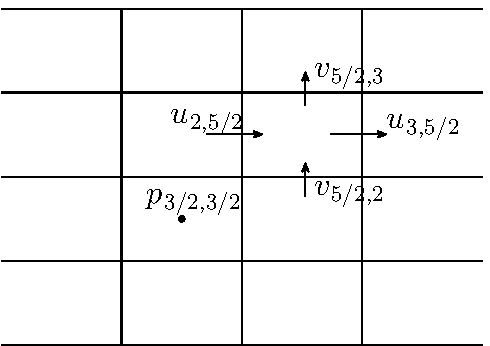
\includegraphics{StaggardGrid}}
\caption{Staggered grid showing the grid points of $u$, $v$ and $p$ field. The horizontal velocity $u$ is defined at the center of vertical faces of cell, vertical velocity $v$ is defined at the center of horizontal faces and the pressure is defined at the center of cell.   }
\label{staggered}
\end{figure}
\begin{equation}
\frac{\tilde{\bu}^{n+1}-\bu^{n}}{\Delta t}+(\bu^n \cdot \grad )\bu^n - \frac{1}{R} \grad^2 \bu^n
\label{TransportEq}
\end{equation}
Where $\Delta t$ is the size of time discretization, n denotes time label and $R$ is the Reynolds number. In the second step, we add pressure gradient operator and impose the incompressibility of flow.
\begin{equation}
\begin{split}
 \frac{\bu^{n+1}-\tilde{\bu^{n+1}}}{\Delta t} +\grad P &= 0\\
 \grad \cdot \bu^{n+1} = 0
 \label{IncompressibleCondEq}
 \end{split}
\end{equation}
Using the staggered grid the two components of \eqref{TransportEq} can be written as
\begin{equation}
\begin{split}
 \tilde{u}_{i,j+1/2}^{n+1} &= u_{i,j+1/2}^n - \Delta t \left(u u_x + vu_y -\frac{1}{R}\grad^2u \right)_{i,j+1/2}^n -\Delta t\Ndg (u^2)_{i,j+1/2}^n\\
 \tilde{v}_{i+1/2,j}^{n+1} &= v_{i+1/2,j}^n - \Delta t \left(u v_x + vv_y -\frac{1}{R}\grad^2v \right)_{i,j+1/2}^n
\end{split}
\end{equation}
where $\left(u u_x + vu_y -\frac{1}{R}\grad^2u \right)_{i,j+1/2}^n$ and $\left(u v_x + vv_y -\frac{1}{R}\grad^2v \right)_{i,j+1/2}^n$
needs to be evaluated at the grid location for the x-component of velocity at $(i,j+1/2)$ and for y-component of the velocity at $(i+1/2,j)$, respectively. The equations \eqref{IncompressibleCondEq} are discretized as 
\begin{equation}
\begin{split}
 u^{n+1}_{i,j+1/2} &= \tilde{u}^{n+1}_{i,j+1/2} -\frac{1}{R} \frac{\Delta t}{\Delta x} \left(p_{i+1/2,j+1/2}^{n+1} -p_{i-1/2,j+1/2}^{n+1} \right)\\
 v^{n+1}_{i+1/2,j} &= \tilde{v}^{n+1}_{i+1/2,j} -\frac{1}{R} \frac{\Delta t}{\Delta y} \left(p_{i+1/2,j+1/2}^{n+1} -p_{i+1/2,j-1/2}^{n+1} \right)
 \end{split}
 \label{true_velocity_cmp}
\end{equation}
where $\Delta x$ and $\Delta y$ are the uniform grid spacing in the x and y directions, respectively. The continuity equation on this staggered can be written as 
\begin{equation}
 \frac{ u_{i+1,j+1/2}^{n+1}-u_{i,j+1/2}^{n+1} }{ \Delta x } +\frac{v_{i+1/2,j+1}^{n+1}-v_{i+1/2,j}^{n+1} }{\Delta y} = 0
 \label{staggered_continuity}
 \end{equation}
Substituting the velocity components from \eqref{true_velocity_cmp} into \eqref{staggered_continuity}, we get discretized poisson equation for pressure.
\begin{equation}
\begin{split}
  \Delta t \left[\frac{p_{i+3/2,j+1/2}^{n+1}-2p_{i+1/2,j+1/2}^{n+1}+p_{i-1/2,j+1/2}^{n+1}}{\Delta x^2} \right] &+
 \Delta t \left[ \frac{p_{i+1/2,j+3/2}^{n+1}-2p_{i+1/2,j+1/2}^{n+1}+p_{i+1/2,j-1/2}^{n+1}}{\Delta y^2}   \right] = \\
 \frac{\left(\tilde{u}_{i+1,j+1/2}^{n+1}-
  \tilde{u}_{i,j+1/2}^{n+1}  \right) }{\Delta x}&+\frac{\left(\tilde{v}_{i+1/2,j+1}^{n+1}-\tilde{v}_{i+1/2,j}^{n+1}  \right)}{\Delta y}
\end{split}
\label{pressure_equation}
\end{equation}
The no-normal velocity on the top and bottom surface provides boundary condition for pressure field, which are used to solve for pressure using \eqref{pressure_equation}. Substitutuing the pressure from the solution of \eqref{pressure_equation} in to \eqref{true_velocity_cmp} we get the velocity field at the next time step. 
\begin{figure}
\centerline{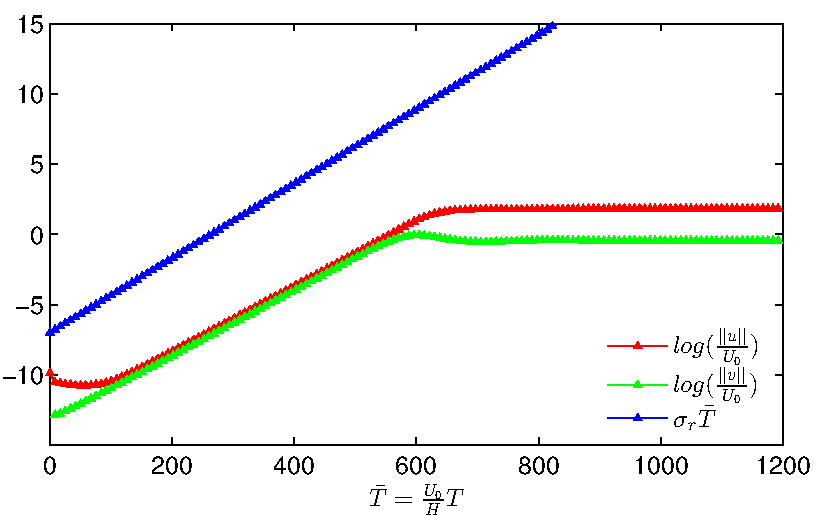
\includegraphics{LinearStabilityVsCFD1} }
\caption{Graph showing growth rate of a random perturbation made to the solution of \eqref{base_equ}, by explicitly solving \eqref{averaged_eq} and its comparison with the highest growth rate predicted by linear stability analysis. The $\sigma_r$ is the real part of growth rate predicted by linear stability analysis. The  Reynolds number, grass number density and submergence ratios are $R=500$, $\Ndg=2$ and $h_{grass}/(2H) = 0.4$ respectively.}
\label{CFD_vs_LinearStabilityGrowthRate}
\end{figure}

We have explicitly solved \eqref{averaged_eq} with the intitial condition $u(x,y,0) = U_{0}(y)+\tilde{u}_0(y)$ and $v(x,y,0)=0$, where $U_{0}(y)$ is velocity profile arising from the solution of \eqref{basicflow} and $\tilde{u}(y) = \epsilon f(y)$ where $\epsilon \ll 1$ and $f(y)$ is an arbitrary function. We expect this perturbation to grow exponentially as $||u(t)|| = ||u(t_0)|| e^{\sigma_r (t-t_0)}$ with the maximum growth rate ($\sigma_r$) as predicted by the solution of \eqref{Orr-somerfield}, where $||.||$ represent $L_2$ norm of perturabation. A comparison of growth rate computed from the solution of \eqref{averaged_eq} with the
maximum growth rate $\sigma_r$ arising from the solution of \eqref{Orr-somerfield} is shown in Figure \ref{CFD_vs_LinearStabilityGrowthRate}, we can see intially when the perturabation to the $U_0(y)$ is small, the perturbation grow with the rate predicted by \eqref{Orr-somerfield}. However once the magnitude of perturbation becomes comparable to the $U_0(y)$, non-linear effect also become important and the growth rate can not be described the solution of linear stability analysis. 

In the regime when $||u-U_0|| \ll ||U_0||$, we also expect that the profiles of perturb velocities $\tilde{u}(x,y,t) = u(x,y,t) - U_0(y)$ and $\tilde{v}(x,y,t) = v(x,y,t)$ can be easily descibed by the dominant eigen mode $\phi(k,y)$ corresoponding to $k$ with the highest growth rate.
\begin{equation}
\begin{split}
 \tilde{u}(x,y,t) &= \Re\left(\phi_y(k,y) e^{ikx+\sigma t+ i\theta}\right)\\
 \tilde{v}(x,y,t) &= \Re\left(ik \phi(k,y) e^{ikx+\sigma t + i\theta }\right)
\end{split}
\end{equation}
Where $\theta$ is a constant phase between $\tilde{u}(0,y,t)$ and $\Re(\phi_y(k,y) e^{\sigma t})$. A comparison between initial evolution of perturb variables $(\tilde{u}, \tilde{v}, \tilde{p})$ with a random perturbation to the base flow $U_0(y)$ arising from the solution of \eqref{averaged_eq} with the prediction based  on the dominant eigen-mode $\phi(k,y)$ is shown in Figure \ref{CFD_vs_LinearStability_AllVariables}

\begin{figure}
\centerline{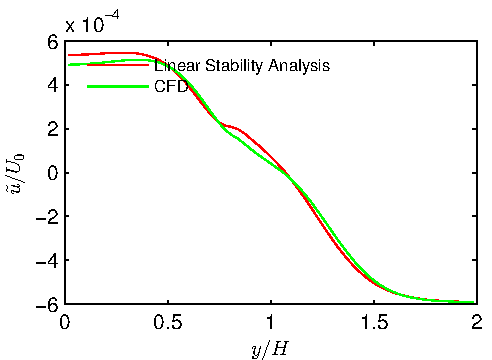
\includegraphics{LinearStabilityVsCFD_u_phase0} 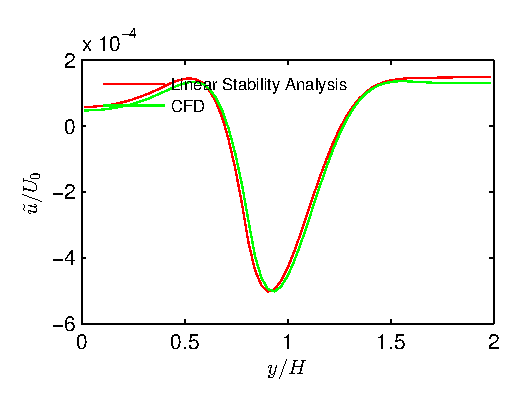
\includegraphics{LinearStabilityVsCFD_u_phase90}}
\centerline{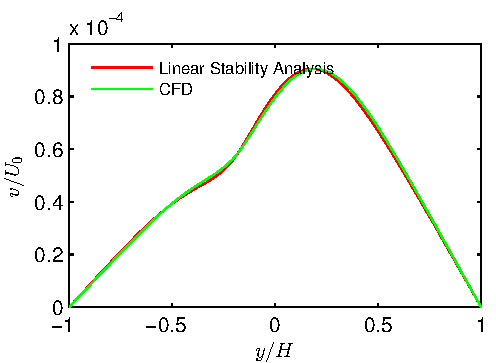
\includegraphics{LinearStabilityVsCFD_v_phase0} 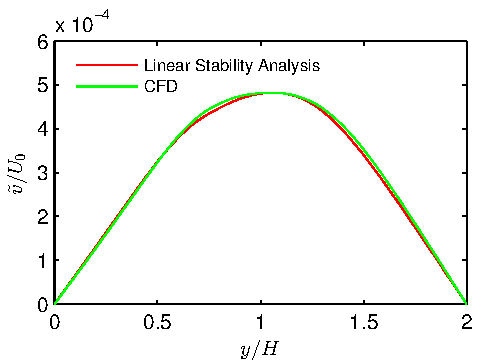
\includegraphics{LinearStabilityVsCFD_v_phase90}}
\centerline{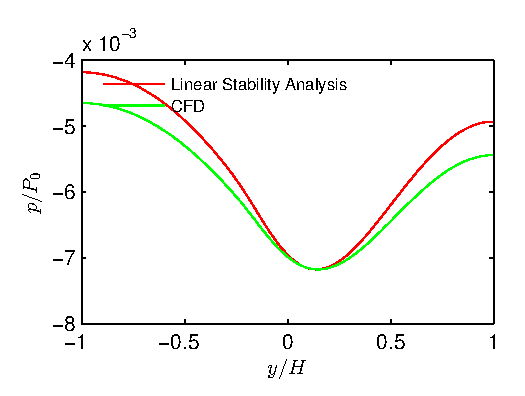
\includegraphics{LinearStabilityVsCFD_p_phase0} 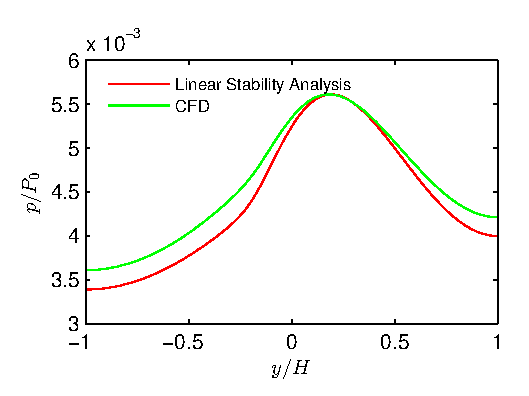
\includegraphics{LinearStabilityVsCFD_p_phase90}}
\caption{Comparison of velocities and pressure predicted by Linear Stability analysis and by explicitly solving \eqref{averaged_eq}. The comparison are made at $\bar{T}=82$ and two different locations, where velocities are $\pi/2$ out of pahse with each other.}
\label{CFD_vs_LinearStability_AllVariables}
\end{figure}
\clearpage{\pagestyle{empty}\cleardoublepage}

\section{Saturated Region}

\begin{figure*}
\centerline{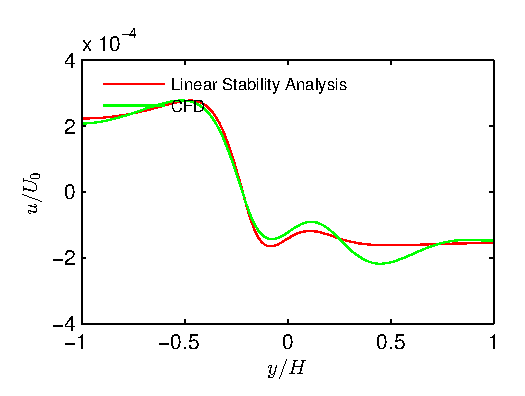
\includegraphics{LinearStabilityVsCFD_Saturated_u_phase0} 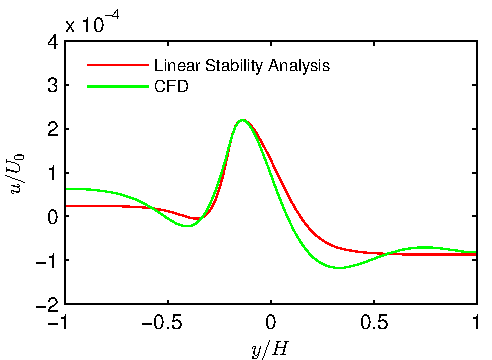
\includegraphics{LinearStabilityVsCFD_Saturated_u_phase90}}
\centerline{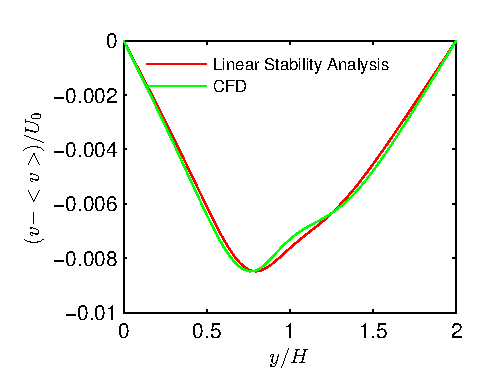
\includegraphics{LinearStabilityVsCFD_Saturated_v_phase0} 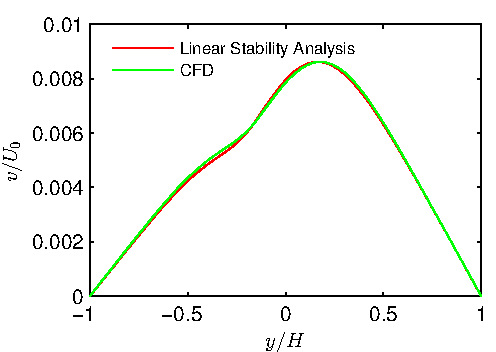
\includegraphics{LinearStabilityVsCFD_Saturated_v_phase90}}
\centerline{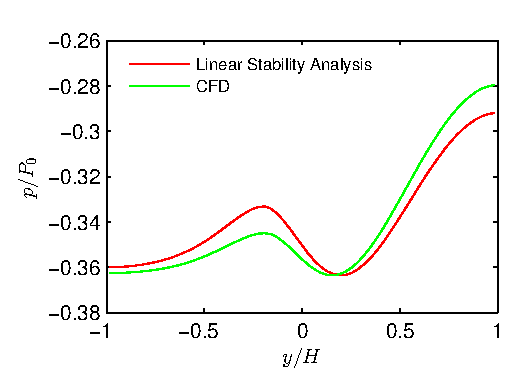
\includegraphics{LinearStabilityVsCFD_Saturated_p_phase0} 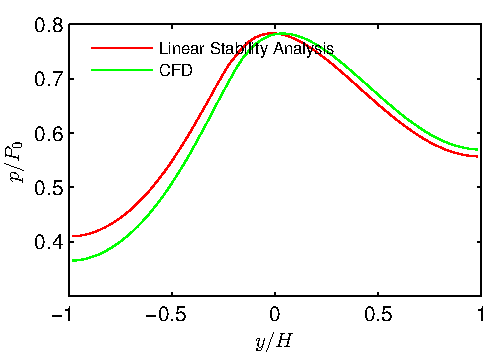
\includegraphics{LinearStabilityVsCFD_Saturated_p_phase90}}
\label{CFD_vs_LinearStability_u}
\end{figure*}







%\lipsum[1-20]

\clearpage{\pagestyle{empty}\cleardoublepage}

%------------------------ APPENDIX ------------------------%
\appendix
\chapter{Stuff Too Complicated To Talk About}
%\lipsum[51-70]

\clearpage{\pagestyle{empty}\cleardoublepage}

\chapter{Stuff Too Boring to Talk About}
%\lipsum[111-130]

\clearpage{\pagestyle{empty}\cleardoublepage}

%---------------------- BIBLIOGRAPHY ----------------------%

\bibliographystyle{plain}
\begin{spacing}{0.9}
  \bibliography{thesis}
\end{spacing}

\end{document}
